%
% PENSER À :
% - vérifier taille de police et interligne
%

\documentclass[a4paper,12pt]{report}

\usepackage[utf8]{inputenc}
\usepackage[T1]{fontenc}
%\usepackage[francais]{babel}
\usepackage[english]{babel}

\addto\captionsenglish{% Replace "english" with the language you use
  \renewcommand{\contentsname}%
    {Table of Contents}%
}

\usepackage[a4paper,top=3cm,bottom=3cm]{geometry}

\usepackage{graphicx}
\usepackage{pdfpages}
\usepackage{float}

\usepackage{fancyhdr}
\pagestyle{fancy}
\renewcommand\headrulewidth{1pt}
\rhead{ \LaTeX }
\cfoot{ \thepage }

\usepackage{titlesec}
\usepackage{hyperref}

% maths
\usepackage{amsmath}
\usepackage{amssymb}
\usepackage{bm}
\newcommand{\prodSc}[2]{\langle #1 / #2 \rangle}
\newcommand{\quSt}[1]{\bm{|#1\rangle}}
\newcommand{\icite}[1]{\up{\textit{\cite{#1}}}}

\titleformat{\chapter}{\normalfont\huge}{\thechapter.}{20pt}{\huge}

\renewcommand{\chaptername}{ }
\DeclareTextFontCommand{\emph}{\bfseries}

\newcommand{\para}[1]{\par{#1}\\}

\title{QUBITS}
\author{QUÉLARD Xavier}
\date{ \today{} }

\makeindex

\usepackage{listings}
\usepackage{color}

\definecolor{dkgreen}{rgb}{0,0.6,0}
\definecolor{gray}{rgb}{0.5,0.5,0.5}
\definecolor{mauve}{rgb}{0.58,0,0.82}

\lstset{frame=tb,
  language=Java,
  aboveskip=3mm,
  belowskip=3mm,
  showstringspaces=false,
  columns=flexible,
  basicstyle={\small\ttfamily},
  numbers=none,
  numberstyle=\tiny\color{gray},
  keywordstyle=\color{blue},
  commentstyle=\color{dkgreen},
  stringstyle=\color{mauve},
  breaklines=true,
  breakatwhitespace=true,
  tabsize=3
}

\begin{document}

%
% -----------------------
% [1] PAGE DE GARDE
% -----------------------
%

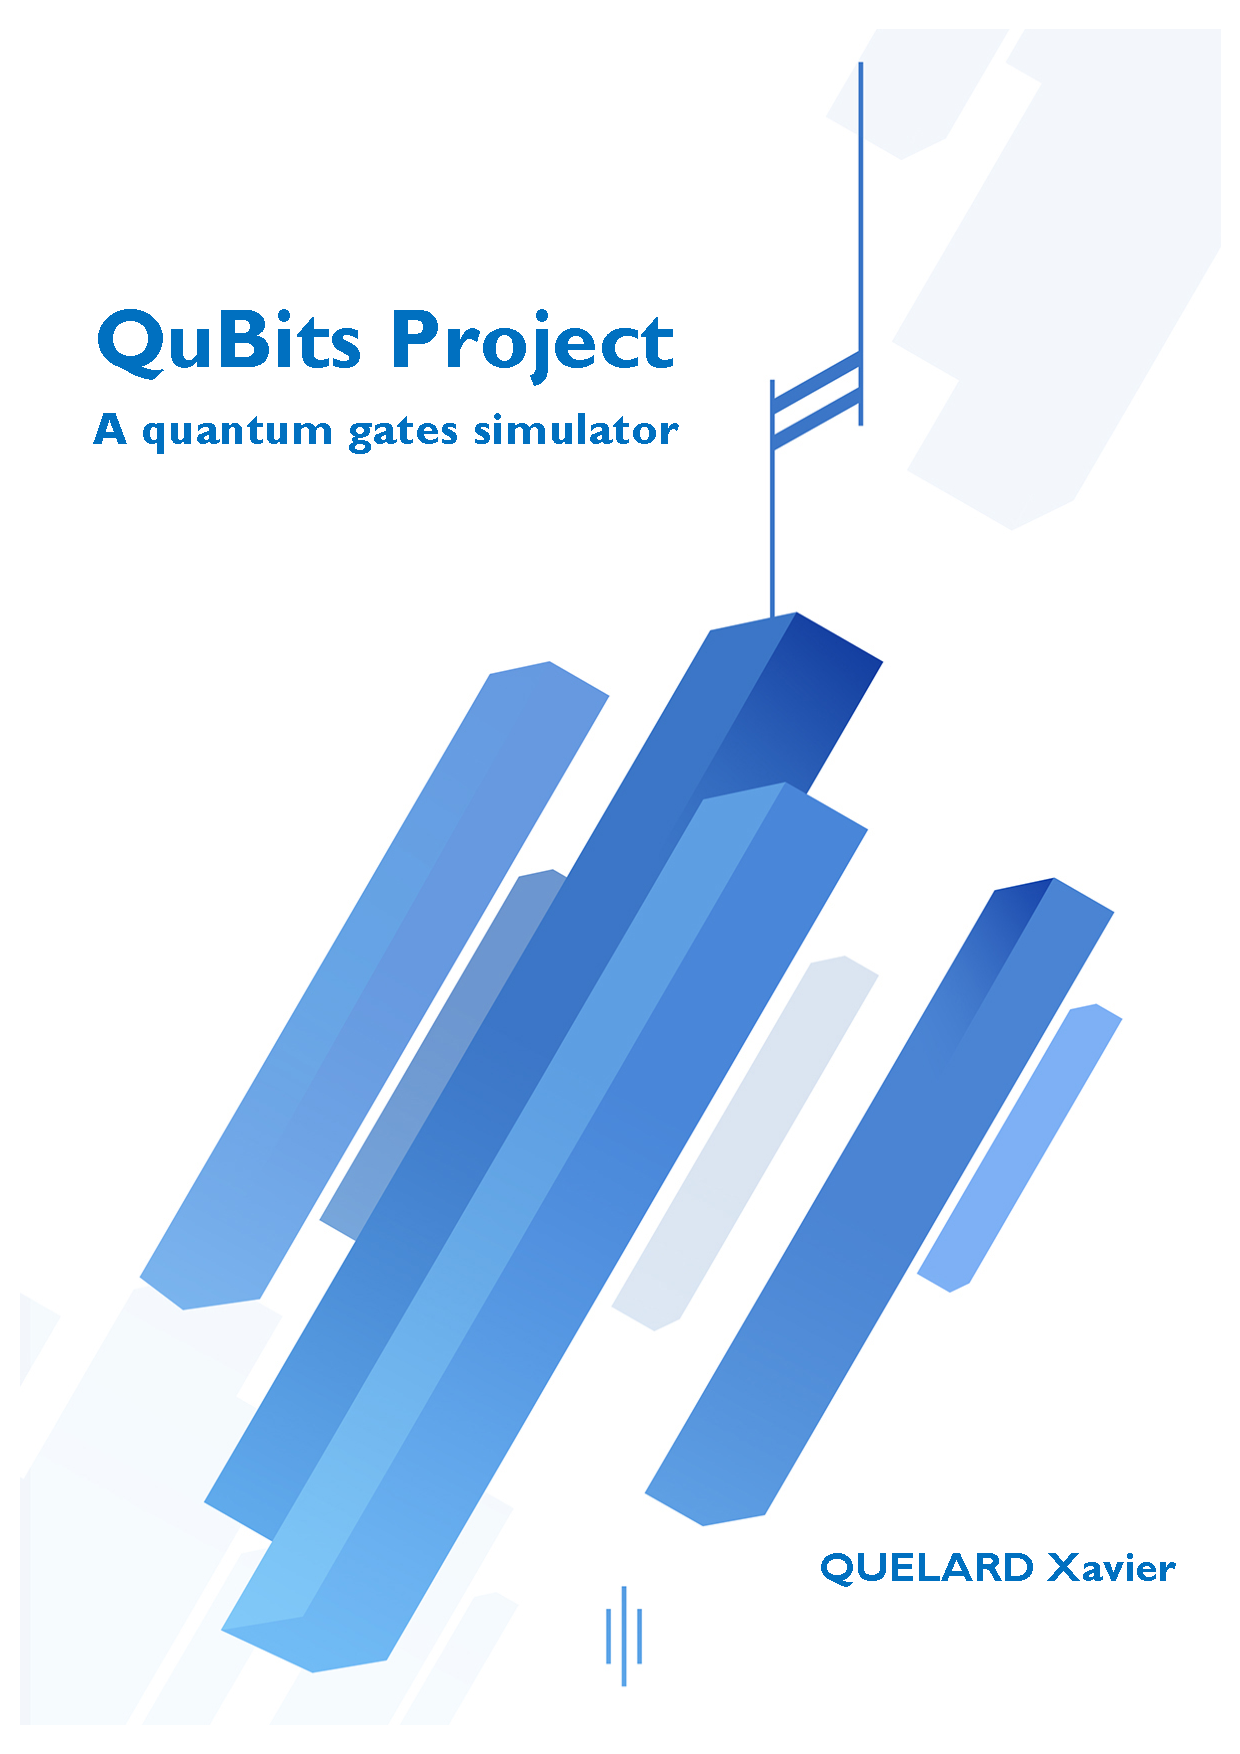
\includepdf{Garde}
%\maketitle

%
% -----------------------
% [2] ToC
% -----------------------
%

\tableofcontents

%
% -----------------------
% [3] Introduction
% -----------------------
%

\chapter{Introduction}

\para{
    Quantum computers are on everyone's lips nowadays. These futuristic computers, built following the strange rules of quantum mechanics, are suppossedly going to be much faster that our current computer. But right now, very few and only very specialised quantum computers even exists.
}

\para{
    But how is a quantum computer supposed to work? What are the rules of the microscopic world? And why quantum computing might be much faster than "classical" computing? That's what will be discussed in the first chapter of this report. A short mathematical background will also be delivered for the most interested lectors. Then, the project QuBits, which consisted of creating a quantum computer simulator, will be explained and detailled, and its results shared and compared to other simulators.
}

%
% -----------------------
% [4] I/ Contexte du projet
% -----------------------
%

\chapter{Project's context}
    \section{History of quantum physics}

\vspace{1\baselineskip}

\para{
    In this very first section of the report, we will focus on the story of quantum physics\icite{bibli1} \icite{bibli2}.
}

\para{
    One could say the first ideas of quantum mechanics were born in 1897, when the physicist Max Planck tries to theorize the black body radiation (see figure \ref{black-body}), a physicist problem that was unsolved at the time. He came with a formula that was describing the reality very accurately, but without any clue on why this was the right answer. Indeed, the physics world was divided between the atomists and the non-atomists, and as one of the latter, Plank was trying to reconstruct his results without atoms.
}

\begin{figure}[H]
	\begin{center}
		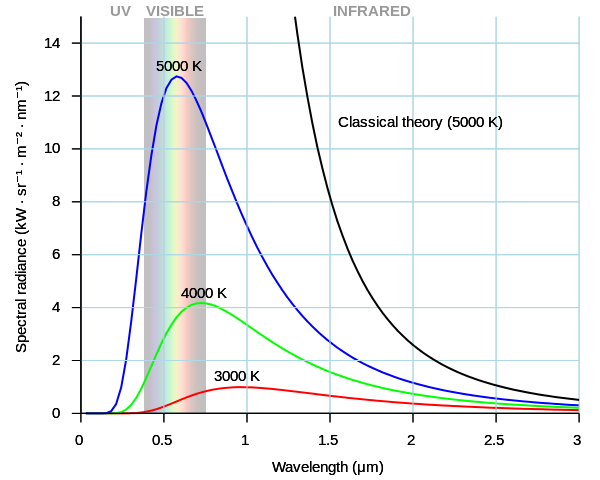
\includegraphics[scale=0.4]{images/black-body}
	\end{center}
	\caption{\textit{The curve Planck was trying to describe and later explain. It basically shows how the wavelength of an object differs with its temperature.}}
	\label{black-body}
\end{figure}

\para{
    After 3 years of hard work, Plank was not able to explain the black body radiations without atoms, so he completely changed his mind on the subject. After another year of reseach, he was able to explain the curve by taking atoms into account. But to successfully derive his mathematical law, he also needed to include more restrictions : atoms can only be at certain levels of energy. He discovered that in the atomic world, energy was discrete, quantified (see figure \ref{atom-energy}).
}

\begin{figure}[H]
	\begin{center}
		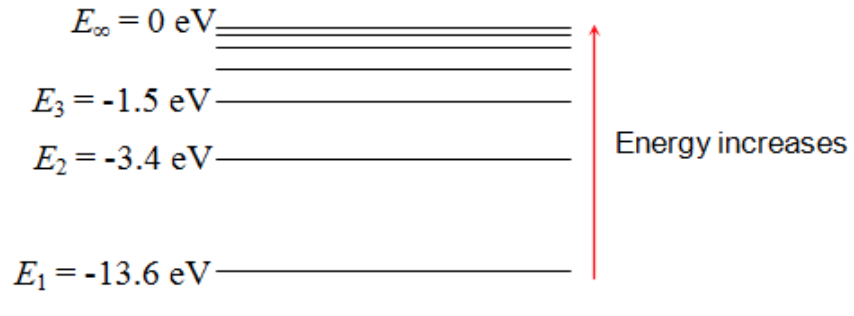
\includegraphics[scale=0.6]{images/atom-energy}
	\end{center}
	\caption{\textit{The curve Planck was trying to describe and later explain. It basically shows how the wavelength of an object differs with its temperature.}}
	\label{atom-energy}
\end{figure}

\para{
    But for five years, not a single paper was written to talk about Plank's quantum ideas. To the more enthusiastics, these ideas were an elegant way to get a mathematical law to work but probably not very realistic, while for the others, it was simply a failure without any sense. That's when a young Albert Einstein wrote his first scientific papers, proving that Plank's theory was not working just for black body radiation, but was a general principal of physics instead, that can and should be applied for a lot of other objects. By applying it to the light, Einstein theorizes the existence of photons, which are small quantums of light. The same way atoms's energy can only have certian values, light's energy is discrete and can be reduced to those particles.
}

\para{
    Albert Einstein's paper could have been laughable form the perspective of the physicists community. But with his photons theory, he was able to explain an effet that was still at mystery at the time : the photoelectric effect (see figure \ref{photoelectric}). Where classical physics failed to give a correct explanation of the phenomenon, the quantified light of Einstein was working very well, and ultimately this paper (among other brilliants one he published in the same time period) won his the Nobel prize later on.
}

\begin{figure}
	\begin{center}
		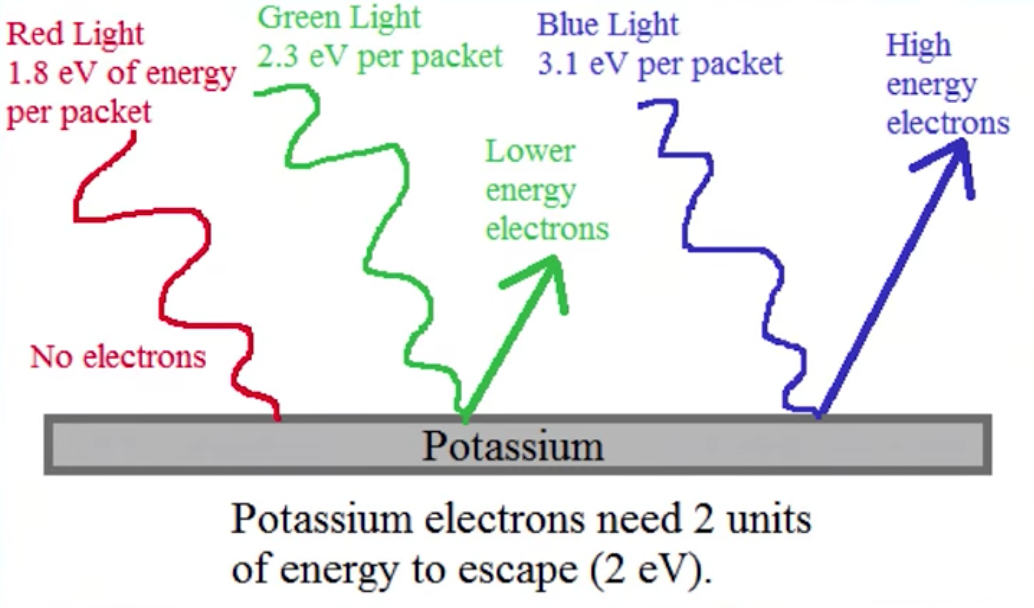
\includegraphics[scale=0.6]{images/photoelectric}
	\end{center}
	\caption{\textit{The photoelectric effect describes how a metal reacts to the emmision of a light, and how it changes electrically speaking depending of the wavelength.}}
	\label{photoelectric}
\end{figure}

\para{
    The next step for the quantum theory was discovered by Neils Bohr in 1912. He was the first scientific able to combine Plank's atom theory and Einstein's light theory to create an atom model. In this model, and atom can jump on or off in energy levels by respectively absorbing or emitting a photon. Depending on the quantity of energy  emitted, a different wavelength of light was obtained (see figure \ref{bohr}). This gave a direct explaination of elements spectroscopy (each element reflects a different discrete spectrum when observed with light).
}

\begin{figure}
	\begin{center}
		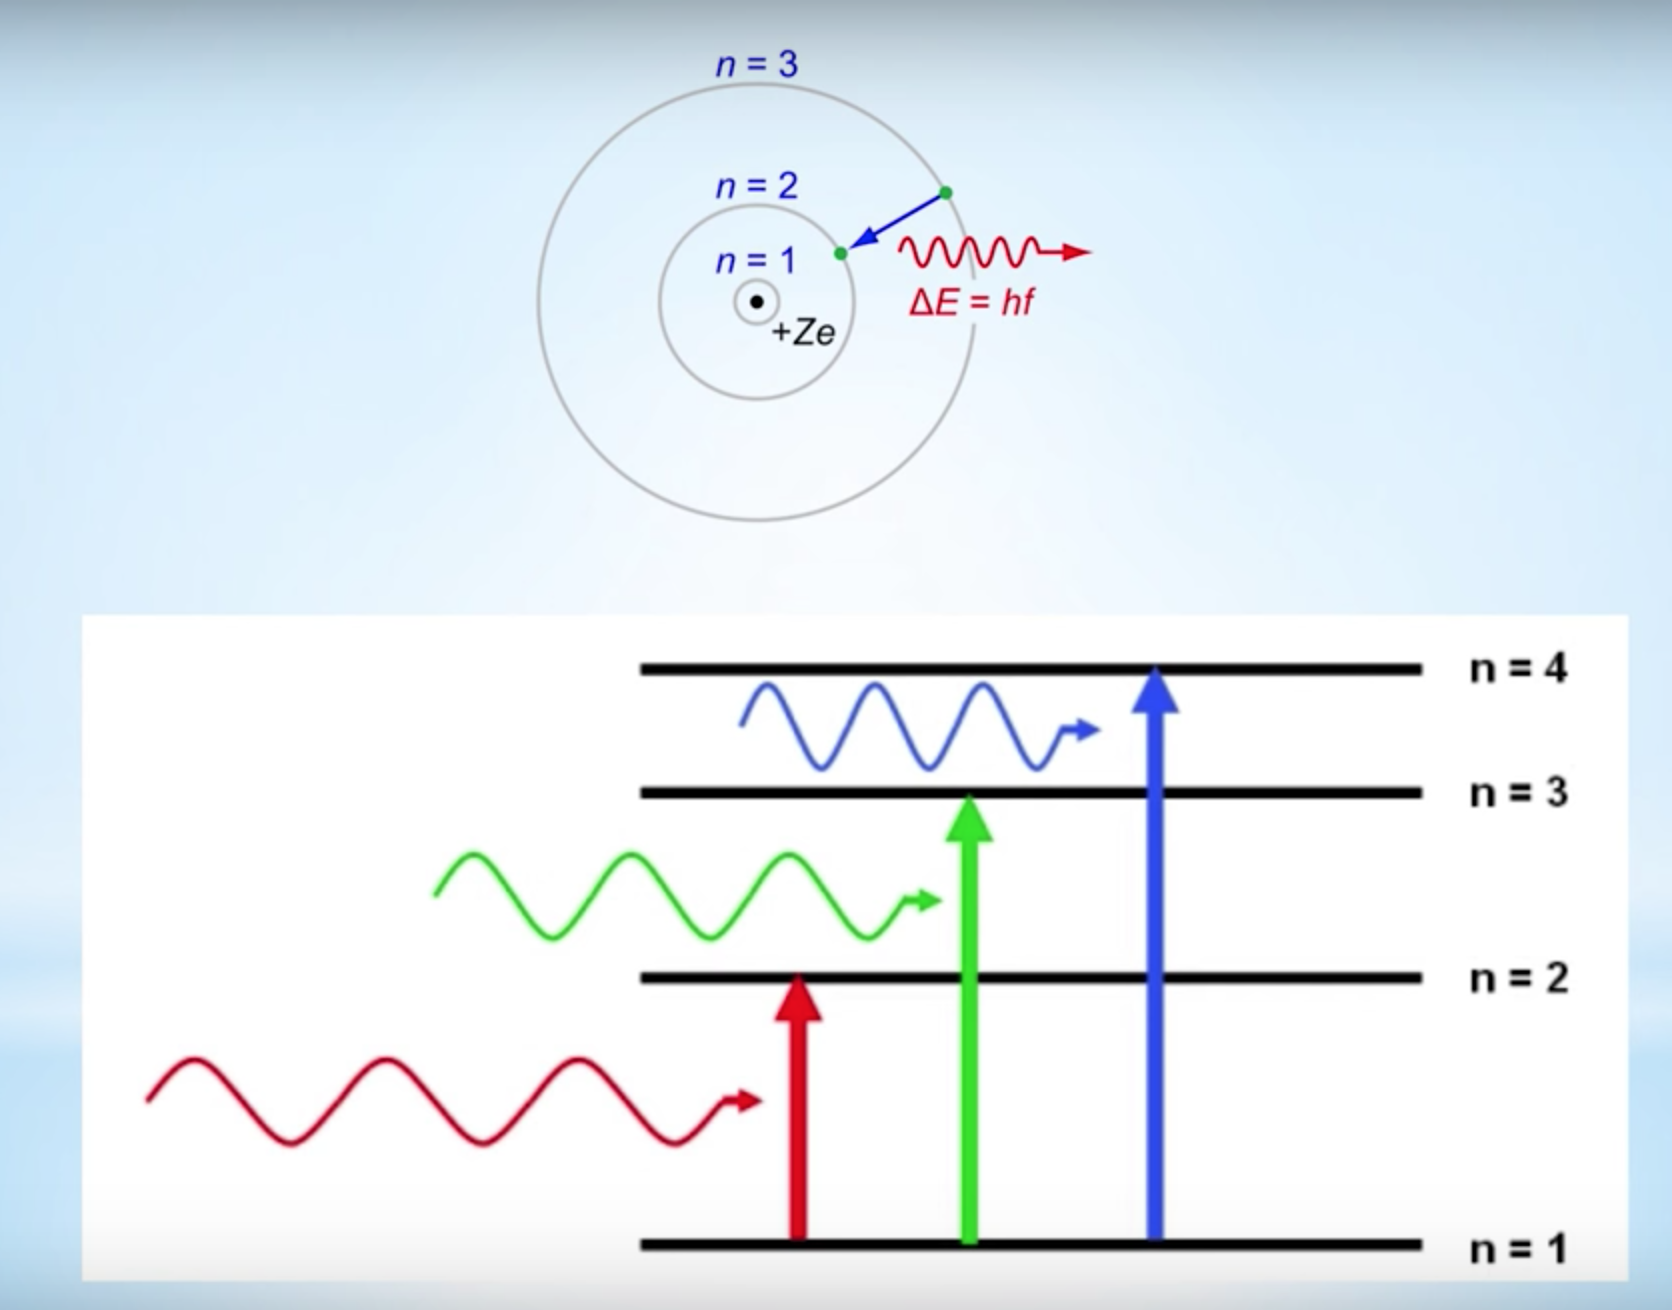
\includegraphics[scale=0.4]{images/bohr}
	\end{center}
	\caption{\textit{The formula relates discrete amount of energy and light's frequency. As frequency and wavelength are inversionally proportionnal, this relation gives a link between energy absorbed by an atom and the spectrum of it. }}
	\label{bohr}
\end{figure}

\para{
    The final step of quantum theory was made by Werner Heisenberg and Erwin Schrödinger in respectively 1925 and 1926. This time, they were not explaining only isolated phenomenon, but based on the previous works of Plank, Einstein and Bohr, they created an equivalent to the prevalent Newton's theory. At the time, these two theories were competing and both better at predicting events than Newton's laws of motion. What was fascinating is that although these two theories were using completely different mathematical objects (matrices and waves), they had incredibly similar results. Years after that, it was in fact mathematically proven that those theories were strictly equivalent, and by no one else than Schrödinger himself.
}

    \section{Quantum physics basic principles}

\para{
    As we have seen previously, quantum theory slowly became accepted in the physicists world, ans as time went on, it proved to be the most successfull theory ever created, explaining and predicting with incredible precision the rules of the atomic realm. Nowadays, it is used in most piece of technologies, and is for example the reason why GPS are so precise. But now that we have learned a bit more about its history, let's dive into its fundamental principles and its strange laws. We will learn about several very important principles of quantum mechanics that we need in order to understand quantum computing. We will discover how counterintuitive most of these are, highlighting that the world does not behave the same way at all in the microscopic scale.
}

        \subsection{Superposition principle} \label{superposition}

\para{
    The first idea is called the superposition principle. While a classical object is too big to follow the quantum mechanics's rules, a quantum object -for example an atom or an electron- follows this superposition principle. A quantum object can be in a superposition of states, which means that instead of having predetermined and fixed variables (position, speed, etc...), it can be in a superposition of very different states. Therefore, an atom might "be" at two places and move at two different speeds at the same time. In quantum theory, a superposition of 4 states is noted like this (this bracket notation is called "ket") :
    \begin{equation}
        \quSt{atom} = \quSt{state1} + \quSt{state2} + \quSt{state3} + \quSt{state4}
    \end{equation}
    A famous illustration of this phenomenon is Schrödinger's cat : an animal that would be both dead and alive according to quantum mechanics.
}

        \subsection{Measurment indeterminism}

\para{
    The second key idea in quantum mechanics is the indeterminism of the measurment. Measuring a quantum object's properties is very different from a macroscopic measurment, because this time, the object may be in several different states. And quantum physics shows that when measuring a quantum object, only one of its many states will be observed, and the outcome is purely random. There is no deterministic law that can tell for sure which state will be "chosen" upon measurment : it is purely and simply random.
}

        \subsection{Quantum states reduction} \label{reduction}

\para{
    However, once one state has been measured, any further measurment will give the same state again 100 percent of the time. This means that not only the measurment is randomly "made" between all the superposed states, but once it is done, the quantum object is in one single state : the measure affects the object it tries to analyse. This is called the reduction of quantum states, as measuring a quantum object reduces him from a superposition of states to a single one (see figure \ref{copenhagen}).
}

\begin{figure}
	\begin{center}
		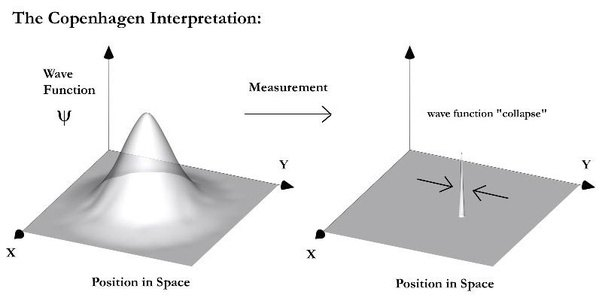
\includegraphics[scale=0.6]{images/copenhagen}
	\end{center}
	\caption{\textit{The Copenhangen interpretation of quantum idea is the most accepted one in the physicists community. Before measurment, a particle can be anywhere on the graph, but as soon as the measure is made, the uncertainty drops and the atom has a single position in space.}}
	\label{copenhagen}
\end{figure}

        \subsection{Particle-wave duality}

\para{
    The fourth key idea in quantum mechanics is the particle-wave duality. It is again a very strange phenomenon that describes the fact that in the quantum world, some objects like electrons behaves like a wave or like a particle, depending on the context. The experiment that showed it was probably the most famous of the 20th centuary : the double vent Feynman experiment. He used a electron cannon to fire electrons, one by one, at a "wall" with two vents and was registering the impacts of the electrons on the backstop. If the two vents are open, interferences figures were appearing on the screen, suggesting that electrons were behaving live waves. On the other hand, opening a single vent was showing electrons shot like gun's bullets, suggesting a particle's behaviour (see figure \ref{feynman}).
}

\begin{figure}
	\begin{center}
		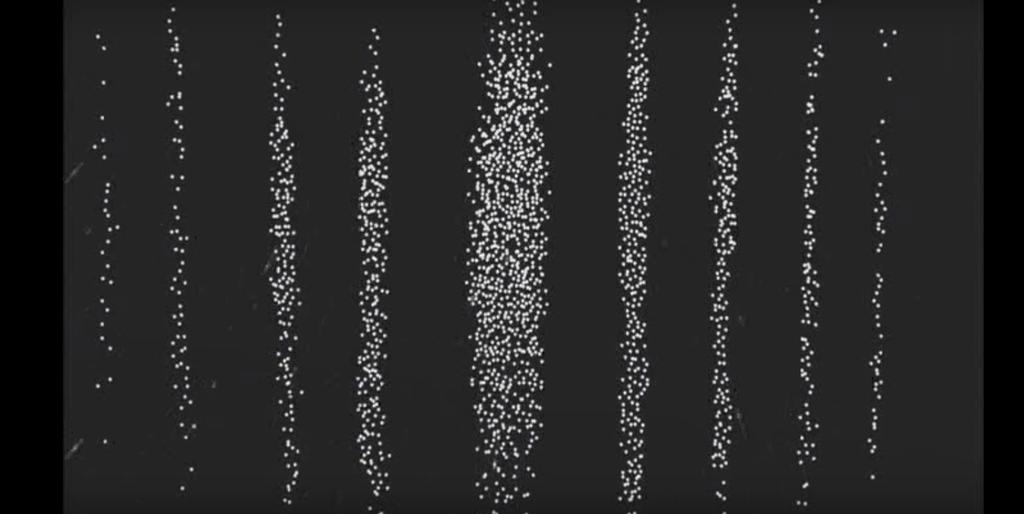
\includegraphics[scale=0.3]{images/feynman}
	\end{center}
	\caption{\textit{Results if the two vents were open. We can clearly see some interferences figures. On the other, with one vent close, a single column of dots would be observed.}}
	\label{feynman}
\end{figure}

        \subsection{Heisenberg uncertainty principle}

\para{
    The last important law of quantum physics that needs to be explained here is the Heinsenberg incertainty principle. It is quite simple but very confusing, as it states that it is impossible to have a quantum state where both position and speed of a particle are well defined at the same time. In fact, the more precise a speed measurment is, the less accuracy there will be on its momentum (equation (\ref{heisenberg}) shows this law for a particle on a single axis position x).
}

\begin{equation}
    \Delta p\Delta x \ge \frac12 \hbar
    \label{heisenberg}
\end{equation}

    \section{Introduction to quantum computing}
        \subsection{Classical computer}

\para{
    In order to understand the project’s stakes, it is important to know how a quantum computer basically works and why it differs from what we call a « classical » computer, which is the type of computer everyone uses nowadays.
    A well known fact is that computers uses electrical signals  to exchange informations. For stability reasons, specialists chose to only code two inputs : 0 and 1, which stands for wether or not there is a signal. It is indeed a clever choice, as it is quite simple to check for only two possibilities that are very distincts. Using those two values, every information is stored in bits, and with clever maths, it is possible to encode anything you can see on a computer : numbers, text, colors, images, etc..
    Calculations are not exceptions, and are also done using bits on classical computers, so every operation has been reprogrammed to work with bits instead of numbers. With a few amount of basic « logical gates » ( = a circuit that takes one or multiple bits and apply a basic operation), addition, then multiplication, and other operations were available to computers.
}

\begin{figure}
	\begin{center}
		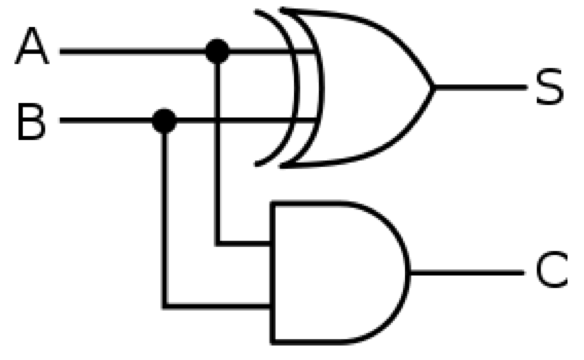
\includegraphics[scale=0.6]{images/adder}
	\end{center}
	\caption{\textit{A circuit that takes A and B as 1-bit inputs, and outputs the sum S and the carry C. It uses only two logical gates, the XOR and AND gates.}}
	\label{copenhagen}
\end{figure}

        \subsection{Quantum computer and project's goals}

\para{
    We have seen that in order to work, a computer basically needs two crucial features :
}

\begin{itemize}
\item[$\bullet$] A way to store and exchange informations, with bits
\item[$\bullet$] A way to apply operations on information, with logical gates
\end{itemize}

\para{
    A quantum computer seems just like a classical computer, doing those same two things, but using quantum bits (or qubits) and quantum gates instead. Basically, a quantum bit is just a bit following the quantum mechanics rules. But as it is ruled by these strange laws, it can perform way better than current computers on few keys problems. As an example, a working quantum computer would be able to search for an entry in a database incredibly faster than a normal one, thanks to its quantum algorithms. Even better : it is mathematically proven that no classical computer can perform better than what we already built, which means the only way to progress in by using quantum devices.
}

\para{
    But for now, working on real qubits is not really possible for anyone but few scientists. Therefore, simulating those qubits is a very real possibility. It can allow scientists to test and discover new algorithms using these QuBits, in order to make progress in computing science. And this is exactly the subject of the QuBits project : to simulate qubits and quantum gates. The goal was to create a program that simulates these two quantum object, and therefore simulate a basic quantum computer.
}

        \subsection{Why is there such an interest on quantum computing?}

\para{
    But a question remains : why is the interest so high in quantum computing? What are its promises? There are two main reasons for that : the first one is quantum computing power, and the second one is quantum algorithms.
}

\para{
    As qubits are quantum objects, they can be in a superposition of states. So while a classical bit would either be in the 0 or 1 state, a qubit can be in a superposition of the states $\quSt{0}$ and $\quSt{1}$, (as seen on part (\ref{superposition}) ). This means that doing an operation on a qubit in both state is like doing two operations on two classical bits. But quantum computers are not just two times "faster" than classical ones : if a register of 2 qubits is used, there is 4 states : $\quSt{00}$, $\quSt{01}$, $\quSt{10}$ and $\quSt{11}$. In general, if you use a register of n qubits, there is $2^n$ states, so if a qubit is in each of these states, the computing power is much greater than a classical computer (see figure (\ref{exponential-power}) ).
}

\begin{figure}
	\begin{center}
		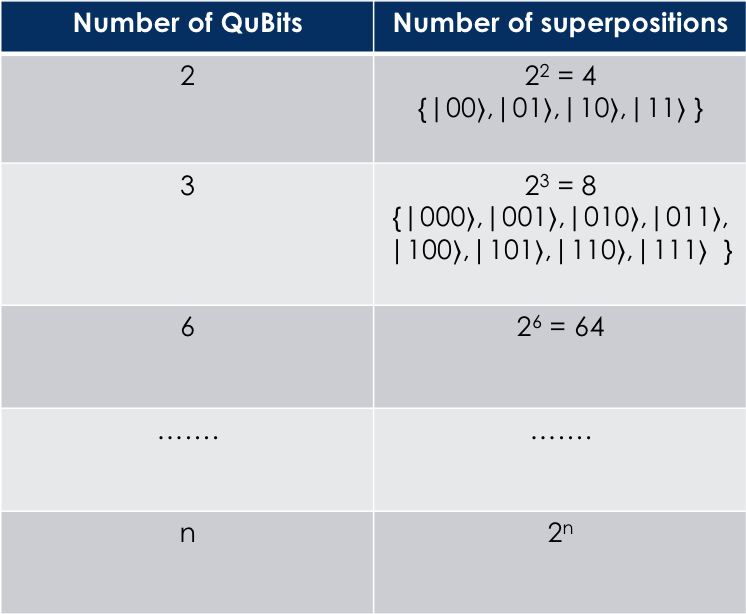
\includegraphics[scale=0.6]{images/exponential-power}
	\end{center}
	\caption{\textit{The number of superpositions explodes when n, the number if qubits, is growing. This exponential growth shows the amazing possibilites brougth by quantum computing.}}
	\label{exponential-power}
\end{figure}

\para{
    However, the quantum state reduction principle (section (\ref{reduction}) ) states that once a measurment is made, a quantum object only stays in one quantum state. This means that although the calculations can be made on each state, only one measure can be made, so only one state will remain. A lot of information can be used during the caculations, but in the end, only one can be kept. It looks a bit like using complex numbers to factorize polynomials : you can use these intermediates to simplify calculations, but in the end, you come back to the real numbers realm, and complex numbers were just an intermediate.
}

\para{
    This is were quantum algorithm comes into place. We will discuss further this point later on, but in order to use quantum computers computing power, algorithm that can work with this measurment limitation needs to be used. Of course, not all problems can be solved this way, and probably most of them will not. But for those where a quantum solution is found, a great acceleration in performances is the reward.
}

\para{
    For example, right now, a lot of cryptography relies on the RSA algorithm\footnote{Rivest Shamir Adleman ares the inventor of this algorithm}. This algorithm make the operation of decrypting a message without the key very difficult, because it relies on the factorisation of two very big prime numbers, an operation that takes an insane amount of time for classical computers. Therefore, a hacker would need million years to hack crypted messages with RSA. However, a quantum algorithm called Shor's algorithm could make the same mathematical operation within seconds. But then, would quantum chips be the end of numerical security? Not really, because it could also bring new ways of crypting messages that would this time be impossible to crack, according to the laws of physics.
}

\para{
    Searching a match in a database is another algorithm that is quite slow on a classical computer. But with Grover's quantum algorithm, a quantum computer could drastically outperform classical computer on this task. While a classical algorithm needs to check every single element of the database (and therefore has a temporal complexity of $O(N)$ operations, where $N$ is the size of the database), Grover's algorithm has a complexity of $O(\sqrt{N})$! On a large database, the computation gains are incredibly high.
}

%
% -----------------------
% [5] II/ Rappels mathématiques
% -----------------------
%

\chapter{Mathematical reminders} \label{Maths}

Most mathematical notions and definitions in this chapter comes from the courses I had during my preparatory classes\icite{ref1}.

    \section{Qubits}
        \subsection{Qubit definition}

\par{
	Let $\mathbb{H}_{n}$ be a Hilbert complex space of $n$ dimensions. Any vector of the $\mathbb{H}_{2}$ space is defined by : $\quSt{\Phi} = \lambda \quSt{0} + \mu \quSt{1}$, where $\lambda$ and $\mu$ are complex coefficients, and $\{\quSt{0}, \quSt{1} \}$ is a orthonormal base (both vectors are orthogonal and normalized). The scalar or dot product of two vectors is then defined by (\ref{prodScH2}), and its norm is defined by (\ref{normeH2}).
}

\begin{equation} \label{prodScH2}
	 \prodSc{\Phi}{\Psi} = \langle ~ \lambda \quSt{0} + \mu \quSt{1} ~/~ \nu \quSt{0} + \sigma \quSt{1} ~\rangle = \lambda^* \nu + \mu^* \sigma = \prodSc{\Phi}{\Psi}^*
\end{equation}

\begin{equation} \label{normeH2}
	 || \Phi ||^2 = \prodSc{\Phi}{\Phi} = \langle ~ \lambda \quSt{0} + \mu \quSt{1} ~/~ \lambda \quSt{0} + \mu \quSt{1} ~\rangle = |\lambda|^2 + |\mu|^2
\end{equation}

\vspace{1\baselineskip}

\par{
	We also add a constraint to each qubit : the normalisation condition (\ref{normalisation}). This will prove to be useful later on.
}

\begin{equation} \label{QuBit}
	\quSt{Q} = \alpha \cdot \quSt{0} + \beta \cdot \quSt{1}
\end{equation}

\begin{equation} \label{normalisation}
	(\alpha,\beta) \in \mathbb{C}^2 ~/~ |\alpha|^2 + |\beta|^2 = 1
\end{equation}

        \subsection{Measuring a qubit}

\par{
	Measuring a qubit\icite{ref2} can be described as a function $\mathbb{M} : \mathbb{H}_{2} \rightarrow \{ \quSt{0}, \quSt{1} \}$ : take a random qubit, and measuring it will either give $\quSt{0}$ state or $\quSt{1}$ state. But as seen previously, measurment is not deterministic in quantum mechanics : in fact, measuring the state $\quSt{Q} = \quSt{0}$ in the $\{\quSt{0}, \quSt{1} \}$ base will give $\quSt{0}$ every single time. Similarly, measuring $\quSt{Q} = \quSt{1}$ will give $\quSt{1}$. However, in the general case, where the qubit in a combination of both states, it becomes trickier. Let $\quSt{Q}$ be a vector of $\mathbb{H}_{2}$. The probability of measuring it in the $\quSt{\Omega}$ state is defined by (\ref{probaState}).
}

\begin{equation} \label{probaState}
	P(~ M( \quSt{Q} ) = \quSt{\Omega} ~) = | \langle ~ \quSt{Q} ~/~  \quSt{\Omega} ~\rangle |^2 = P(~ M( Q ) = \Omega ~)
\end{equation}

\vspace{1\baselineskip}

\par{
	So, for a given qubit $\quSt{Q} = \alpha \cdot \quSt{0} + \beta \cdot \quSt{1}$, it has $\lambda^2$ chances of being measured in the $\quSt{0}$ state, and $\mu^2$ chances of being in the $\quSt{1}$ state. This is where the normalisation (\ref{normalisation}) suddenly makes quite a lot of sense. This works for sure as long as a orthonormal base is chosen.
}

        \subsection{Bloch's sphere}

\par{
	The goal of this subsection is to give the lector a visual representation of a quantum state. In order to do so, the Bloch's sphere shall be introduced. Let's examine the following equivalence relation $R : \mathbb{H}^2 \rightarrow \mathbb{H}^2$ \\
}

\begin{equation}
	 \quSt{\Psi} R \quSt{\Psi '} \Leftrightarrow \exists z \in \mathbb{C} / \left\{
		  \begin{array}{rcr}
		      \quSt{\Psi} R \quSt{\Psi '} \Leftrightarrow \quSt{\Psi} = z \quSt{\Psi '} \\
		      |z| = 1 \\
		  \end{array}
		\right
\end{equation}

\par{
	$R$ trivially verifies reflexivity, symetry et and transitivity. Belonging to the same equivalence class means the qubits are all equals except for a phase factor  $z = e^{i\theta}$. We can then obserb that multiplying a state by a phase factor doesnt change its probability of being measured in a given $\quSt{\alpha}$ state :
}

\begin{align}
	P(~ M( z \quSt{\Psi} ) = \quSt{\alpha} ~) &= \prodSc{z \quSt{\Psi}}{\quSt{\alpha}} \\
	 &= |e^{i\theta}| \prodSc{\quSt{\Psi}}{\quSt{\alpha}} \\
	 &= P(~ M( \quSt{\Psi} ) = \quSt{\alpha} ~)
\end{align}

\vspace{1\baselineskip}

\par{
	This means that two qubits can be considered equals if belonging to the same equivalence class, which leads to the following rewriting :
}

\begin{align}
	\label{blochEq}
	\forall \quSt{\Psi} \in \mathbb{H}^2 , \exists \theta \in [0, \pi] ~/~ \quSt{\Psi} &= \cos(\theta/2) \cdot \quSt{0} + \sin(\theta/2) e^{i(\varphi)} \cdot \quSt{1} \\
	&\equiv \cos(\theta/2) e^{-i(\varphi/2)} \cdot \quSt{0} + \sin(\theta/2) e^{i(\varphi/2)} \cdot \quSt{1}
\end{align}

\vspace{1\baselineskip}

\para{
    With this new equation, it is possible to represent even single qubit (with the phase factor ignored) on a sphere, where $\theta$ and $\varphi$ are the colatitude and the longitude (see figure (\ref{bloch}) ). There is a isomorphism between the qubit space and the Bloch's sphere. However, one may say that this sphere is only a visual representation : linearity is NOT preserved, as we know $\quSt{0} \neq -\quSt{1}$. This Bloch's sphere is just here to help visualizing the state of a qubit.
}

\begin{figure}
	\begin{center}
		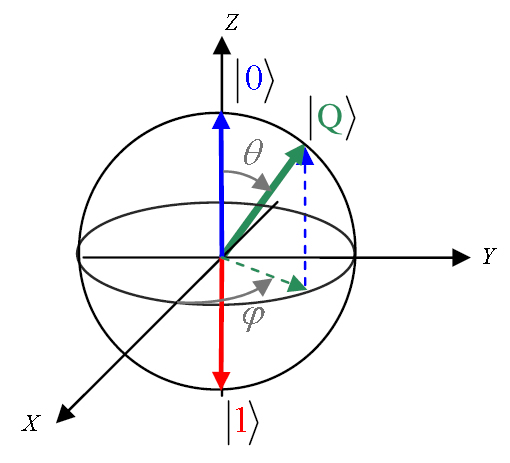
\includegraphics[scale=0.60]{images/bloch}
	\end{center}
	\caption{\textit{Visualizing a quantum state with Bloch's sphere.}}
	\label{bloch}
\end{figure}

        \subsection{Multiple qubits register}

\para{
	Here is defined the tensorial product $\otimes$ of two qubits (\ref{tensoriel}) .
}

\begin{equation}
	\label{tensoriel}
	(\cdot) \otimes (\cdot) : \left\{
	  \begin{array}{rcr}
	    \mathbb{H}^2 \times \mathbb{H}^2 \rightarrow \mathbb{H}^4 \hfill \\
	    (\quSt{\varphi},\quSt{\Psi}) \mapsto \quSt{\varphi} \otimes \quSt{\Psi} = \left( \begin{array}{c} \alpha \\ \beta \\\end{array} \right ) \otimes \left( \begin{array}{c} \lambda \\ \mu \\ \end{array} \right ) = \left( \begin{array}{c} \alpha \lambda \\ \alpha \mu \\ \beta \lambda \\ \beta \mu \end{array} \right ) \\
	  \end{array}
	\right
\end{equation}

\para{
	With this product\icite{ref4} of two $\mathbb{H}^2$, we can define the space of two qubits (so with up to 4 quantum states) :
}

\begin{equation}
	 \{ \quSt{0_A \otimes 0_B}, \quSt{0_A \otimes 1_B} , \quSt{1_A \otimes 0_B} , \quSt{1_A \otimes 1_B} \} = \{ \quSt{00}, \quSt{01}, \quSt{10}, \quSt{11} \}
\end{equation}

\begin{equation}
	 =  \left\{ \left( \begin{array}{c} 1 \\ 0 \\ 0 \\ 0 \end{array} \right ), \left( \begin{array}{c} 0 \\ 1 \\ 0 \\ 0 \end{array} \right ), \left( \begin{array}{c} 0 \\ 0 \\ 1 \\ 0 \end{array} \right ), \left( \begin{array}{c} 0 \\ 0 \\ 0 \\ 1 \end{array} \right ) \right\} \\
\end{equation}

\vspace{1\baselineskip}

\begin{equation}
	 =  \left\{ \left( \begin{matrix} 1 & 0 \\ 0 & 0 \end{matrix} \right ), \left( \begin{matrix} 0 & 1 \\ 0 & 0 \end{matrix} \right ), \left( \begin{matrix} 0 & 0 \\ 1 & 0 \end{matrix} \right ), \left( \begin{matrix} 0 & 0 \\ 0 & 1 \end{matrix} \right ) \right\} \\
\end{equation}


    \section{Quantum gates}
        \subsection{One qubit gates}

\par{
	A quantum gate can be described as a function $L$ :
}

\begin{align}
	\label{porteLogique}
	L( ... ) : \left\{
	  \begin{array}{rcr}
	    \mathbb{H}^{\otimes n} \times \mathbb{H}^{\otimes n} \times \mathbb{H}^{\otimes n} \times ... &\rightarrow \mathbb{H}^{\otimes n} \times \mathbb{H}^{\otimes n} \times \mathbb{H}^{\otimes n} \times ... \hfill \\
	    (\quSt{\varphi }, \quSt{\Psi }, \quSt{\Omega }, ... ) &\mapsto (L(\varphi),L(\Psi),L(\Omega), ...) \\
	  \end{array}
	\right
\end{align}

\par{
    It's simply a linear function which takes several qubits as entry, and outputs the same qubits, modified. Since a quantum gates does not make any measurment, the transformation needs to maintain the normalisation condition. Therefore, we can simply modelize a quantum gate with a matrix $M$ (norm = 1). The state after the gate can then be measured by $L(\Psi) = M \cdot \Psi$ . \\
    By definition, quantum calculus is reversible, which means every quantum gate matrix must be reversible.
}

\par{
    We are now able to define two one-qubit gates : phase $L_{\Phi}$ and rotation $L_{\alpha}$. Let's call $Mat()$ the function that maps the matrix corresponding to a quantum gate (we position ourself in the $\{ \quSt{0}, \quSt{1} \}$ orthonormal base). Then :
}

\begin{equation}
	 Mat(L_{\Phi}) = \left( \begin{matrix} 1 & 0 \\ 0 & e^{i\Phi} \end{matrix} \right ) \\
\end{equation}

\begin{equation}
	 Mat(L_{\alpha}) = \left( \begin{matrix} cos(\alpha) & sin(\alpha) \\ -sin(\alpha) & cos(\alpha) \end{matrix} \right ) \\
\end{equation}

\vspace{1\baselineskip}

\par{
	The first gate adds a phase factor to the $\quSt{1}$ while the second once makes a rotation of $\alpha$. Here are two other gates :
}

\begin{equation}
	 Mat(NOT) = \left( \begin{matrix} 0 & 1 \\ 1 & 0 \end{matrix} \right ) \\
\end{equation}

\begin{equation}
	 Mat(HADAMARD) = \frac{1}{\sqrt{2}} \left( \begin{matrix} 1 & 1 \\ 1 & -1 \end{matrix} \right ) \\
\end{equation}

\vspace{1\baselineskip}

\par{
	The $NOT$ gate is just like the not gate of classical computer. However, the hadamard gate in unique to quantum computing.The goal of this gate is to balance the $\quSt{0}$ and $\quSt{1}$ weights of a given qubit.
}

        \subsection{Two qubits gates}

\par{
	The $CNOT = Controlled \text{ } NOT$ gate is a $NOT$ gate, but acting on the targeted qubit only. The second qubit is named the controlled qubit, and is here to apply a if-statement : if the controlled qubit is in the $\quSt{1}$ state, then apply $NOT$ on the targeted qubit. Otherwise, this gate does nothing. The $CPHASE$ gate will work the same way, applying the $PHASE$ gate on the targeted qubit only if the condition on the controlled qubit is met. Finally, the swap gate simply "exchange" the values of the two qubits it takes.
}

\begin{equation}
	 Mat(CNOT) = \left( \begin{matrix} 1 & 0 & 0 & 0 \\ 0 & 1 & 0 & 0 \\ 0 & 0 & 0 & 1 \\ 0 & 0 & 1 & 0 \\ \end{matrix} \right ) \\
\end{equation}

\vspace{1\baselineskip}

\begin{equation}
	 Mat(CPHASE) = \left( \begin{matrix} 1 & 0 & 0 & 0 \\ 0 & 1 & 0 & 0 \\ 0 & 0 & 1 & 0 \\ 0 & 0 & 0 & e^{i\Phi} \\ \end{matrix} \right ) \\
\end{equation}

\vspace{1\baselineskip}

\begin{equation}
	 Mat(SWAP) = \left( \begin{matrix} 1 & 0 & 0 & 0 \\ 0 & 0 & 1 & 0 \\ 0 & 1 & 0 & 0 \\ 0 & 0 & 0 & 1 \\ \end{matrix} \right ) \\
\end{equation}

%
% -----------------------
% [5] III/ Développement du projet
% -----------------------
%

\chapter{Project's development}

\para{
    Now that we have all the historical and mathematical background needed to understand quantum computers, we will discuss how the project was done, step by step.
}

    \section{Establishing a golden model}

        \subsection{Class diagram}

\para{
    The very first step of the project was to understand how quantum computers should work in theory, in order to develop a simulator. For this reason I wrote a detailled report (in french) about quantum computer's mathematics than can be found in the appendix. The previous chapter (\ref{Maths}) was a shorter version of this document, as its goal was only to give a minimal and condensed mathematical background to the lector.
}

\para{
    The first development step was then to create a golden model of the qubits simulator. A golden model is a first implementation of a program. Its goal is to be implemented quickly in order to allow for the first tests and further refinments. As such, it is also preferrable to use a high-level programming language to benefit from its more readable syntax and shorter development time.
}

\para{
    Before choosing any language, a class diagram of the simulator was established, in order to define once and for all the structure of the simulator. The diagram shown on the figure (\ref{class-diagram}) is the final result.
}

\begin{figure}
	\begin{center}
		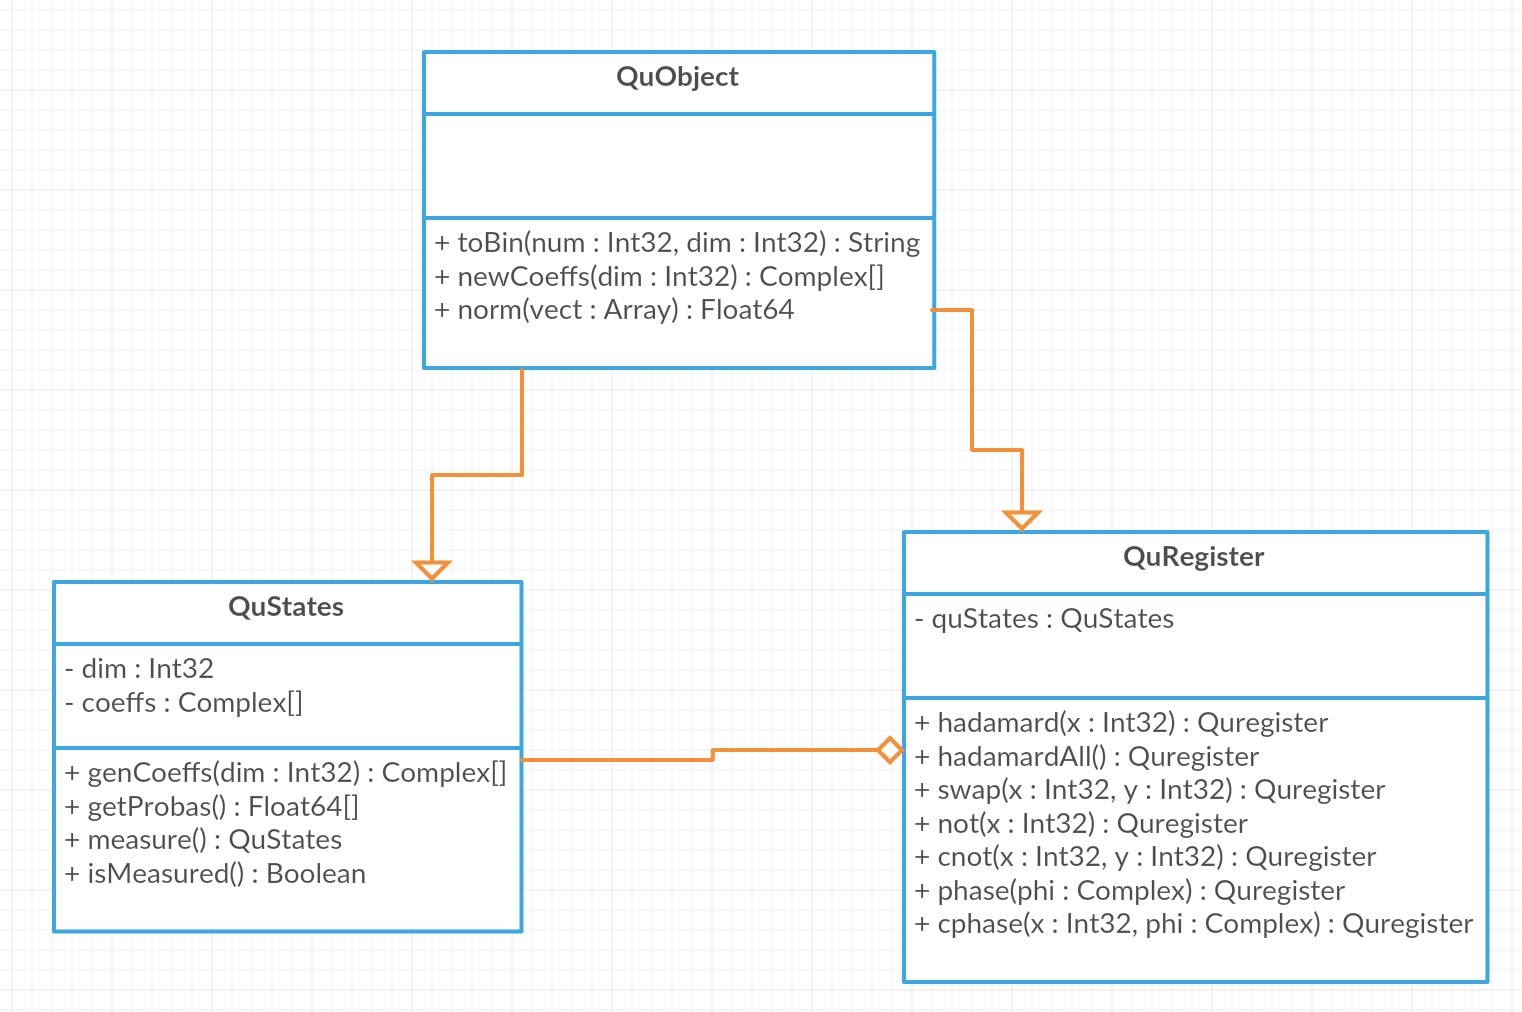
\includegraphics[scale=0.6]{images/class-diagram}
	\end{center}
	\caption{\textit{The projet's class diagram, divided in three main classes. Most important methods are shown, but some like getter and setters and internal operations are hidden for clarity purposes.}}
	\label{class-diagram}
\end{figure}

\para{
    The first class, called QuObject, is an abstract class which only goal is to be inherited by the two others in order for these to share the same structures and have the same basic operations. It contains a string to binary convertion method (the simulator allow users to define qubits with strings rather than vectors, so this operation is needed everywhere in the simulator), but also a norm method (useful for calculating probabilities) and an Int to Complex conversion method, as the user can enter real or complex numbers as parameters of a qubit, but the simulator needs only Complex numbers to work.
}

\para{
    The second class, called QuStates, is a container. It saved all the informations needed for a register of several qubits (or only one qubit) : the dimension and the complex coefficients of each superposed state. And then it provides a measurment method, which uses the getProbas method to simulate a random measurment.
}

\para{
    The last class QuRegister, is the object the user interacts with. Therefore, it has several constructors (either the user instanciate with a string, or with an array of complex numbers) which convert the data and register it in a single QuStates container. Then, this class offers a lot of method for the user to act on the QuState : the quantum gates. Since the QuRegister contains one QuStates on which it acts, there is an aggregation between these two classes.
}

\para{
    It is interesting to point out that each quantum gates return a QuRegister. This is a programming idea that allows the user to chain the quantum gates method calls, like seen in the figure (\ref{chaining}).
}

\begin{figure}[H]
	\begin{center}
		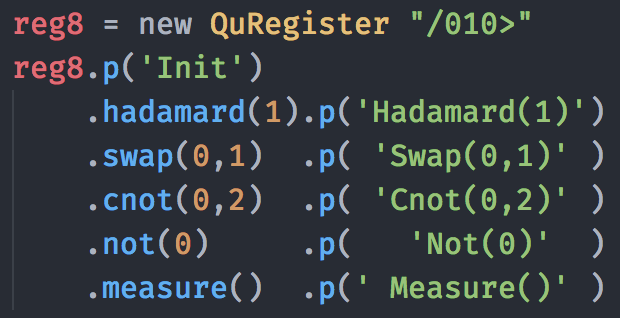
\includegraphics[scale=0.6]{images/chaining}
	\end{center}
	\caption{\textit{Method calls are chained because each method return the this/self object. The p method between each quantum gate called is here to print a text, in order for the user to get a understandable chain of results.}}
	\label{chaining}
\end{figure}

        \subsection{First implementation in Coffescript}

\para{
    Once the object-oriented model was defined, a language to program it had to be chosen. Since the goal was to develop a golden model, the choice was made on Coffeescript. Indeed, Coffeescript is :
}

\begin{itemize}
\item[$\bullet$] A small language that compiles into Javascript, with the goal of giving it a simpler syntax.
\item[$\bullet$] A way of writing object-oriented Javascript with an elegant syntax (very close to a language like Ruby) and a very easy to read language.
\item[$\bullet$] An "extension" of Javascript. Javascript is a multi-platform web language that has a very easy-to-use object-oriented philosophy, simplifying the development of the golden model.
\end{itemize}

\para{
    As a simple, very readable and easy language to use, Coffeescript was a good high level language choice to create the golden model. The source code of the golden model can be found in the appendix.
}

    \section{Development of a more advanced simulator}
        \subsection{Programming language's choice}

\para{
    For the final implementation of the project, another language needed to be used, in order to gain performances. Mr Lelann suggested an emerging new language called Crystal. Crystal is :
}

\begin{itemize}
\item[$\bullet$] A compiled language, therefore way more performance oriented.
\item[$\bullet$] A Ruby-inspired syntax language, which goes quite far, as most of simple Ruby programs can directly be converted into Crystal without changing anything.
\item[$\bullet$] An emerging language than is not very well know nor very well documented.
\end{itemize}

\para{
    The first two points are what lead to the descision of using the Crystal language : with a Ruby-like syntax, converting and enhancing the code from Coffescript would be fast and both codes would look quite similar structurally speaking, while hopefully allowing for some performance gains. However, the last point was the reason why this transition was not immediate. To even use the fundamental libraries, it was often necessary to check Crystal's own source code as the API itself is very lackluster in terms of comments and explanations.
}

        \subsection{Implementation}

\para{
    On the other hand, it was a difficult but pleasant experience to discover a whole new very interesting language by experimenting, looking into the source code and scarce documentation. The final implemention in Crystal can be found in the appendix.
}

%
% -----------------------
% [5] IV/ Algos quantiques et résultats
% -----------------------
%

\chapter{Quantum algorithms and experimental results}

\para{
    In this part of the report, we will introduce several well known quantum algorithms and how they are overperforming classical computers. The Deutsch-Jozsa algorithm will be more detailled as I was able to implement it on the QuBits quantum simulator.
}

    \section{Deutsch-Jozsa algorithm}
        \subsection{Description}

\para{
    Let $f : \{0,1\}^n \mapsto \{0,1\}$ be a function either balanced (equally gives 0 or 1 as an output) or constant (always return 0 (resp. 1)). The Deutsch-Jozsa algorithm is a quantum algorithm that allows a quantum computer to determine whether such a f is balanced or constant with a single operation (while a classical algorithm would need at worst to check half of the function's values to decide). The figure (\ref{deutsch}) shows the quantum circuit of this algorithm.
}

\begin{figure}[H]
	\begin{center}
		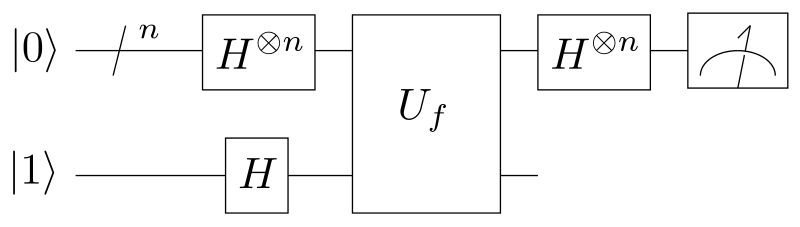
\includegraphics[scale=0.3]{images/deutsch}
	\end{center}
	\caption{\textit{Deutsch-Jozsa algorithm's quantum circuit. }}
	\label{deutsch}
\end{figure}

\para{
    First, you form a n+1 qubits register $\quSt{000...0001}$ where there is n zeros. You then apply the Hadamard gates to all those qubits. The $U_f$ oracle can then be applied : it only changes the very last qubits, applying the operation $f(x) \oplus q$, where $q$ is the current value of the qubit and $\oplus$ is an addition modulo 2. Finally, the Hadamard gate is applied once again, and you measure the first $n$ qubits. If there are only zeros, the $f$ function is constant. In any other case, it is balanced.
}

        \subsection{Implementation}

\para{
    The figure (\ref{deutsch-implementation}) shows the implementation in Crystal of this algorithm. We simply create the $(n*1)$ dimensions qubits (here, $n = 2$), then we apply the oracle between two Hadamard-all gates, and we measure the result.
}

\begin{figure}[H]
	\begin{center}
		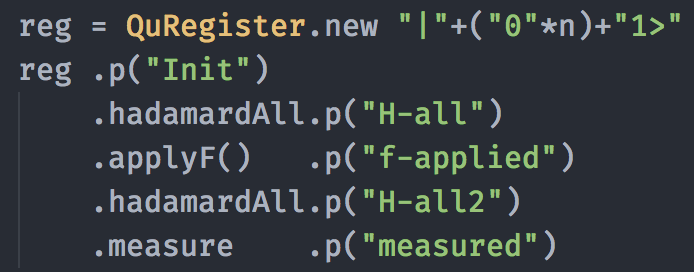
\includegraphics[scale=0.6]{images/deutsch-implementation}
	\end{center}
	\caption{\textit{Deutsch-Jozsa implementation. Method calls are chained thanks to the object oriented structure chosen in the golden model. }}
	\label{deutsch-implementation}
\end{figure}

    \section{Shor and Grover's algorithms}
        \subsection{Shor's algorithm}

\para{
    The Shor's algorithm\icite{bibli3} is a very famous quantum algorithm that solves the prime factorisation problem : given a natural number $N$, find its prime factors. The problem cannot be solved better than with a sub-exponential time complexity with a classical-only algorithm. It has been proved that Shor's algorithm solves the same problem with a ($O(log(N))$) time complexity! With such a superior speed, the factorisation problem brought by the RSA algorithm could be brute forced in a very reasonable amount of time. The figure (\ref{shor}) shows the quantum part of the algorithm.
}

\begin{figure}[H]
	\begin{center}
		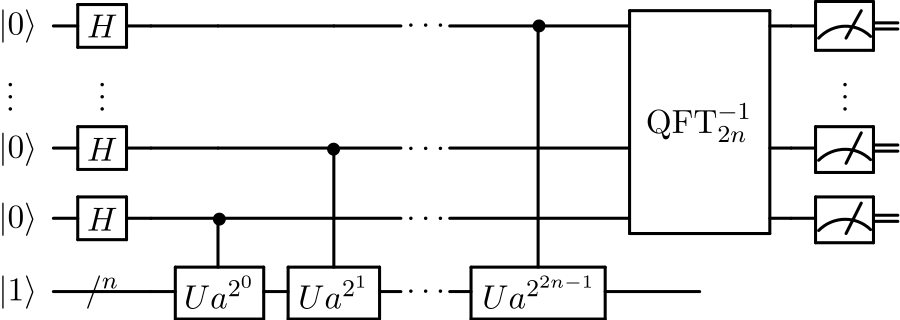
\includegraphics[scale=0.3]{images/shor}
	\end{center}
	\caption{\textit{Shor's algorithm quantum circuit. The difficult part is the implementation of the quantum Fourier transformation, which is quite complicated. }}
	\label{shor}
\end{figure}

        \subsection{Grover's algorithm}

\para{
    Grover's\icite{bibli4} algorithm solves the problem of finding an specific element in a dataset with a very high probability. Any classical algorithm will have at best a $O(N)$ time complexity (where $N$ is the size of the dataset) because in the worst case, the last element is the searched one. However, Grover's algorithm can find a match with high accuracy with a complexity of $O(\sqrt(N))$. Furthermore, four other mathematicians\footnote{Bennett, Bernstein, Brassard, and Vazirani} proved that Shor's algorithm, is asymptotically optimal, which means that no other quantum algorithm could perform better concerning this problem.
}

\begin{figure}[H]
	\begin{center}
		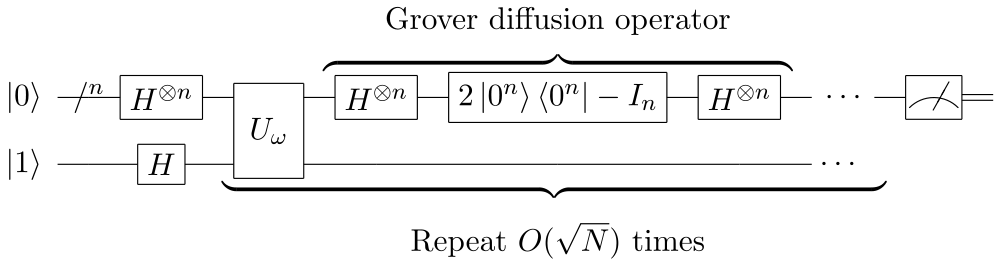
\includegraphics[scale=0.3]{images/grover}
	\end{center}
	\caption{\textit{Grover's algorithm quantum circuit. The difficult part is the implementation of the Grover diffusion operator. }}
	\label{grover}
\end{figure}

\para{
    While Deutsch-Jozsa algorithm is deterministic (it will always give the right answer given the correct inputs), Grover's algorithm is probabilistic. But by iterating it multiple times, it is possible to get the probability of having a correct result insanely close to 1, which is acceptable.
}

    \section{Experimental results}

\para{
    In this last section, we will take a look at the QuBits simulator performances and compare it to its previous iteration, but also to other and more complete quantum libraries.
}

        \subsection{Comparison with other libraries}

\para{
    The most advanced work done with the project's simulator was the implementation of the Deutsch-Jozsa algorithm. To compare the project's simulator with other libraries, I decided to run this algorithm on different solutions and compare the execution times. I chose the javascript library "jsqubits" as my implementation and structure was very similar to this one, thus making the re-implementation of the DJ algorithm much easier. The second library I chose was "qubiter", a Python 3 library. The figure (\ref{results}) shows how these three solutions compares to each other.
}

\begin{figure}
	\begin{center}
		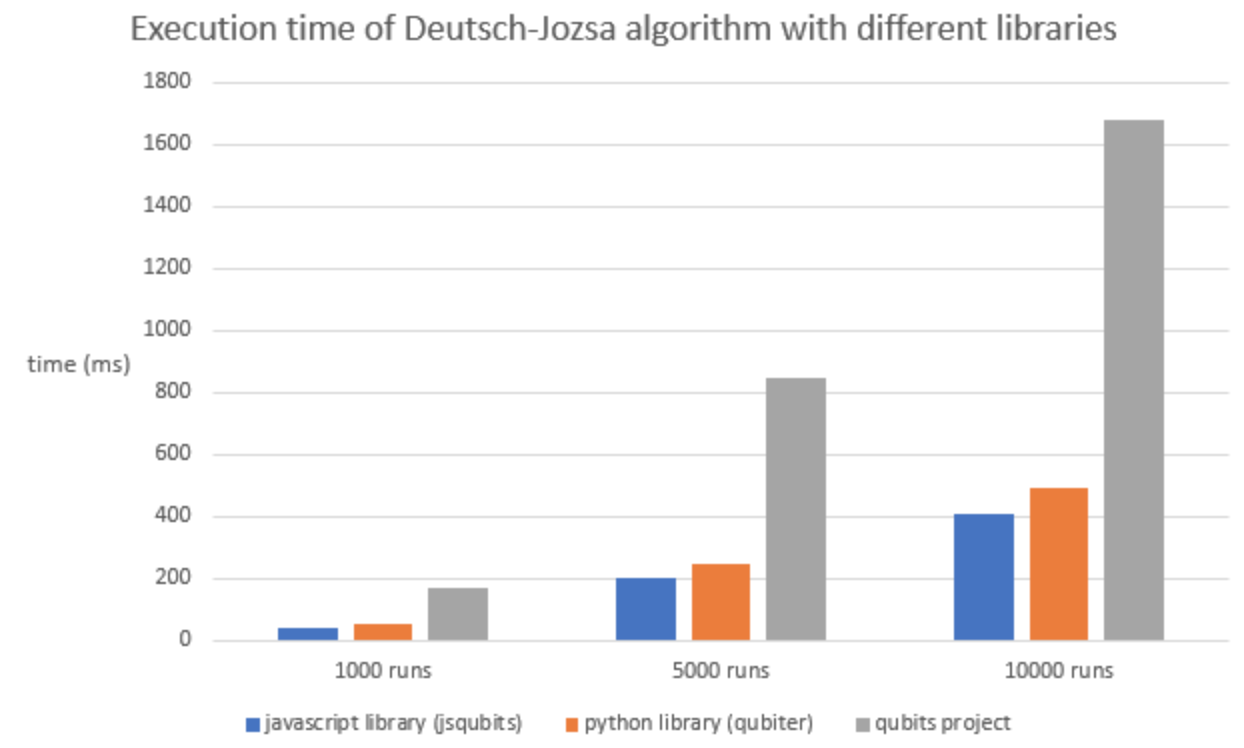
\includegraphics[scale=0.6]{images/results}
	\end{center}
	\caption{\textit{Three libraries compared on their execution time. }}
	\label{results}
\end{figure}

\para{
    As expected, the Javascript and Python libraries work quite faster than the project's Crystal solution. On average, QuBits's simulator was 3.7 times slower than the two others libraries. However, this is not a bad result for a minimalist library made from-scratch by a single student, and without any particular optimization other than changing the programming language from Javascript to Crystal. \\ In conclusion, even thougth other libraries outperform the project's final implementation, these three solutions are relatively on the same scale of execution time (less than a single miliseconds to run the DJ algorithm once).
}

        \subsection{Comparison with the previous implementation}

\para{
    But another interesting comparison would be between the first implementation of the project (the golden model in coffeescript) and the last one (the final result with Crystal). Since the golden model was developped early during the project, it was not yet an option to implement quantum algorithm (the project's goal was initially to simply modelize quantum gates). Therefore, the golden model and the final model cannot be compared on the DJ algorithm execution. However, we can instead compare them on the execution time of the hamadard gate. The figure (\ref{results2}) shows the results of this experiment.
}

\begin{figure}
	\begin{center}
		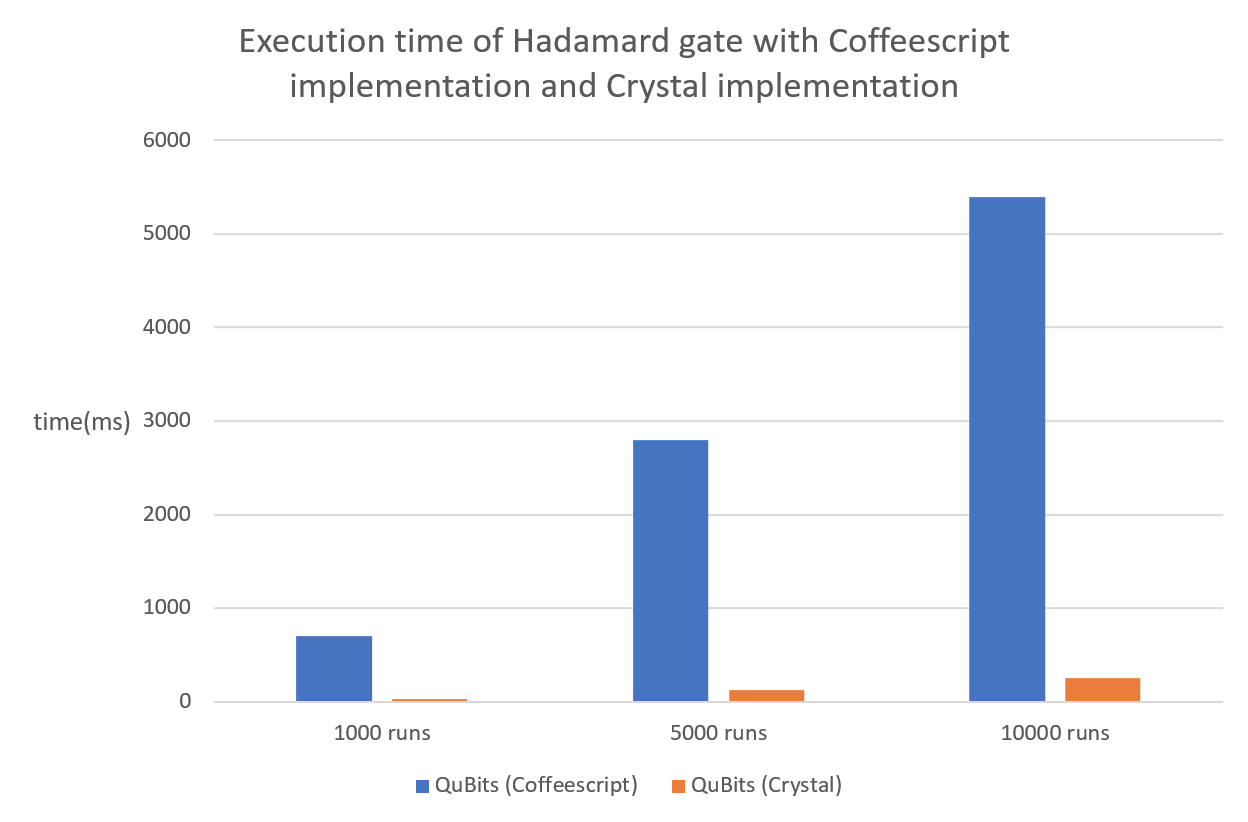
\includegraphics[scale=0.6]{images/results2}
	\end{center}
	\caption{\textit{Comparing the execution time of Hadamard gate between the first and the last implementation of the QuBits project.}}
	\label{results2}
\end{figure}

\para{
    The results are this time extremely clear : the final version of the project is, on average, 24.2 times faster than the golden Coffeescript model! This illustrates very well how a smarter implementation and the use of a compiles language can accelerate caculations. While the final model takes 0.1 second to run the Hadamard gate 5000 times, the golden model asks for almost three seconds to do the same task!
}

%
% -----------------------
% [6] IV/ Conclusion
% -----------------------
%

\chapter{Conclusion}

\para{
    Diving into the strange world of quantum mechanics and computers was a fascinating experience. I was thrilled to learn so many aspects of this topic by myself, and very proud of being able to implement -if not the hardest one- a quantum algorithm with my simulator. I also learned a new language, Crystal, that is very promising for 2018 and very pleasant to use.
}

\para{
    The pleasure I had to make the reseach part of this Project confirms my desire of working in the same way in my future engineer career : a thesis in the quantum computing world would be ideal to me and corresponds to how I like to spend my working time.
}

%
% -----------------------
% [NNNN] Bibliographie
% -----------------------
%

%\chapter*{Bibliography}

\begin{thebibliography}{1}
    \addcontentsline{toc}{chapter}{Bibliography}

    \bibitem{bibli1} \url{https://en.wikiversity.org/wiki/Quantum_mechanics/Timeline} Quantum physics timeline, wikiversity, march 2018
    \bibitem{bibli2} \url{https://www.youtube.com/watch?v=oQYsqnRYb_o} TED Talk The Crazy History of Quantum Mechanics | Leonard Mlodinow, feb 2016
    \bibitem{bibli3} \url{https://en.wikipedia.org/wiki/Shor%27s_algorithm} Shor's algorithm, Wikipedia, march 2018
    \bibitem{bibli4} \url{https://en.wikipedia.org/wiki/Grover%27s_algorithm} Grover's algorithm, Wikipedia, march 2018
    \bibitem{ref1} Mathematics courses of Mr Quibel (Descartes Highschool), second year, Tours, 2014
	\bibitem{ref2} \url{http://dept-info.labri.fr/~ges/ENSEIGNEMENT/CALCULQ/polycop_calculq.pdf} Introduction to quantum conmputing, Y. Leroyer et G. Senizergues, 2016-2017
	\bibitem{ref3} \url{http://stla.github.io/stlapblog/posts/BlochSphere.html} Bloch's sphere, stlaPBlog, Dec 2015
	\bibitem{ref4} \url{http://stla.github.io/stlapblog/posts/JonctionQuantique.html} Junction of two quantum systems, stlaPBlog, Fev 2016
	\bibitem{ref5} \url{https://tel.archives-ouvertes.fr/tel-00180890/document}
\end{thebibliography}

\chapter*{Appendix}
\addcontentsline{toc}{chapter}{Appendix}

\section{Golden model source code (Coffeescript)}

\lstset{language=Ruby}
\begin{lstlisting}
math = require 'mathjs'

class QuObject
    constructor: () ->

    # (array a#, array a2) -> (float |<a1/a2>|^2)
    prodSc: (a1,a2) ->
        math.norm( math.dot(a1,a2) )^2

    # "00010010" -> [0,0,0,1,0,0,1,0]
    getArr: (str) ->
        ret = []
        for i in [0...str.length]
            ret.push( parseInt(str[i]) )
        ret

    # [0,0,0,1,0,0,1,0] -> "00010010"
    getStr: (arr) ->
        ret = ""
        for i in [0...arr.length]
            ret +=  "" + arr[i] + ""
        ret

    toBin: (int, dim) ->
        bin = int.toString(2)
        for i in [0...(dim - bin.length)]
            bin = "0" + bin
        bin

    strReplace: (str, index, replacement) ->
        str.substr(0, index) + replacement + str.substr(index + replacement.length)


# this class represents the quantum state of a register of qubits
class QuState extends QuObject
    # we suppose coeffs.length == dim
    # dim is needed, coeffs might be optional, measured is a boolean
    constructor: (@dim, coeffs = [], @measured = false) ->
        super()
        @coeffs = if (coeffs.length == 0) then ( @genCoeffs(@dim) ) else coeffs
        @coeffs = math.multiply( 1/math.norm(@coeffs), @coeffs ) #normalization

    # (int dim) -> (array complex [a1, ... an]) / n = 2^dim
    genCoeffs: (dim) ->
        [ret, reals, ims] = [ [], math.random([1,@dim])[0], math.random([1,@dim])[0] ]
        for i in [0...Math.pow(2,@dim)]
            ret.push( math.complex(reals[i],ims[i]) )
        ret

    # (QuState state) -> (QuState postMeasureState = finalState)
    getProbas: () ->
        #array of the probability of each state to be measured, the random choice, a sum, and the future return result
        probas = []
        for i in [0...Math.pow(2,@dim)]
            # c'est pas propre mathématiquement mais ça marche et c'est + rapide
            probas.push( Math.pow( math.norm([@coeffs[i]]),2 ) )
        probas

    # return the state after measurment
    measure: () ->
        [probas, choice, sum, result] = [ @getProbas(), math.random(), 0, [] ]
        #console.log 'CHOICE : ' + choice
        for i in [0...Math.pow(2,@dim)]
            [prevSum, sum] = [sum, sum+probas[i]]
            result.push( if(choice >= prevSum && choice <= sum) then 1 else 0 )
        #console.log 'RESULT : [' + result + ']'
        new QuState(@dim, result, true)

    # if the state is measured, return the value of the n-th bit.
    getQubit: (n) ->
        if (!@measured)
            false
        else
            @coeffs[n-1]

    getCoeffs: () ->
        @coeffs

    getState: () ->
        ret = ''
        for i in [0...Math.pow(2,@dim)]
            if math.norm(@coeffs[i]) != 0
                ret += '(' + @coeffs[i] + ')*|' + (@toBin i, @dim) + '> + '
        ret.slice(0,-2)

    isMeasured: () ->
        @measured


class QuRegister extends QuObject
    # give "|001>", "/001>", or [0,1,0,0,0,0,0,0], which represents the same state
    constructor: (st) ->
        super()
        if ( (st[0] == "|") || (st[0] == "/") )  &&  ( st[(st.length)-1] == ">" )
            bin = st.slice(1,(st.length)-1)
            dim = bin.length
            arr = ( 0 for [1..(Math.pow(2,dim))] )
            arr[parseInt(parseInt(bin,2))] = 1
        else
            dim = parseInt Math.log2(st.length)
            arr = st

        @quState = new QuState dim, arr


    getState: () ->
        @quState.getState()

    p: (st) ->
        console.log '[' + st + '] '+ @getState()
        @


    measure: () ->
        #replace the quState with its value after measurment
        @quState = @quState.measure()
        @


    hadamard: (x) ->
        dim = @quState.dim
        newCoeffs = ( 0 for [1..(Math.pow(2,dim))] )

        for i in [0...(Math.pow(2,dim))]
            bin = (@toBin i, dim)
            if (bin[x] == '0') # H(|0>) = ( 1/sqrt(2) )*( |0> + |1> )
                [c1,c2] = [bin, (@strReplace bin, x, "1" )]
                console.log "1/ " + c1 + " -- " + c2
                newCoeffs[parseInt(c1,2)] += (@quState.coeffs[i]/Math.sqrt(2))
                newCoeffs[parseInt(c2,2)] += (@quState.coeffs[i]/Math.sqrt(2))
            else # H(|1>) = ( 1/sqrt(2) )*( |0> - |1> )
                [c1,c2] = [(@strReplace bin, x, "0" ), bin]
                console.log "2/ " + c1 + " -- " + c2
                newCoeffs[parseInt(c1,2)] += (@quState.coeffs[i]/Math.sqrt(2))
                newCoeffs[parseInt(c2,2)] -= (@quState.coeffs[i]/Math.sqrt(2))

        @quState = new QuState dim, newCoeffs
        @


    hadamardAll: () ->
        for i in [0...@quState.dim]
            @hadamard i
        @


    swap: (x, y) ->
        dim = @quState.dim
        newCoeffs = ( 0 for [1..(Math.pow(2,dim))] )

        for i in [0...(Math.pow(2,dim))]
            bin = (@toBin i, dim).split('')
            [ bin[x], bin[y] ] = [ bin[y], bin[x] ]
            bin = bin.join('')
            newCoeffs[parseInt(bin,2)] = @quState.coeffs[i]

        @quState = new QuState dim, newCoeffs
        @


    not: (x) ->
        dim = @quState.dim
        newCoeffs = ( 0 for [1..(Math.pow(2,dim))] )

        for i in [0...(Math.pow(2,dim))]
            bin = (@toBin i, dim)
            if (bin[x] == "0") # NOT(|0>) = |1>
                bin = @strReplace(bin, x, "1")
            else # NOT(|1>) = |0>
                bin = @strReplace(bin, x, "0")
            newCoeffs[parseInt(bin,2)] += @quState.coeffs[i]

        @quState = new QuState dim, newCoeffs
        @


    cnot: (x,y) ->
        dim = @quState.dim
        newCoeffs = ( 0 for [1..(Math.pow(2,dim))] )

        for i in [0...(Math.pow(2,dim))]
            bin = (@toBin i, dim)
            if (bin[x] == "1")
                if (bin[y] == "0") # NOT(|0>) = |1>
                    bin = @strReplace(bin, y, "1")
                else # NOT(|1>) = |0>
                    bin = @strReplace(bin, y, "0")
            newCoeffs[parseInt(bin,2)] += @quState.coeffs[i]

        @quState = new QuState dim, newCoeffs
        @


    phase: (x,phi) ->
        dim = @quState.dim
        newCoeffs = ( 0 for [1..(Math.pow(2,dim))] )

        for i in [0...(Math.pow(2,dim))]
            bin = (@toBin i, dim)
            if (bin[x] == "1")
                newCoeffs[parseInt(bin,2)] = math.multiply(math.complex({r : 1, phi : phi}), @quState.coeffs[i])
            else
                newCoeffs[parseInt(bin,2)] = @quState.coeffs[i]

        @quState = new QuState dim, newCoeffs
        @


    cphase: (x,y,phi) ->
        dim = @quState.dim
        newCoeffs = ( 0 for [1..(Math.pow(2,dim))] )

        for i in [0...(Math.pow(2,dim))]
            bin = (@toBin i, dim)
            if (bin[x] == "1" && bin[y] == "1")
                newCoeffs[parseInt(bin,2)] = math.multiply(math.complex({r : 1, phi : phi}), @quState.coeffs[i])
            else
                newCoeffs[parseInt(bin,2)] = @quState.coeffs[i]

        @quState = new QuState dim, newCoeffs
        @


# testing measure()
reg0 = new QuRegister [math.complex(0,4),0,0,4,0,0,0,0]
console.log "before measure : " + reg0.getState()
reg0.measure()
console.log "after  measure : " + reg0.getState()

# testing hadamard
reg1 = new QuRegister [1,0,0,0,0,0,1,0]
console.log "HADAMARD(0) : " + reg1.getState() + " ---> " + reg1.hadamard(0).getState()

# testing hadamard on all qubits
reg2 = new QuRegister [1,0,0,0,0,0,1,0]
console.log "HADAMARD ALL : " + reg2.getState() + " ---> " + reg2.hadamardAll().getState()

# testing swap on qubits 0 and 2
reg3 = new QuRegister "|001>" # = [0,1,0,0,0,0,0,0]
console.log "SWAP(0,2) : " + reg3.getState() + " ---> " + reg3.swap(0,2).getState()

# testing not on qubit 0
reg4 = new QuRegister "|001>"
console.log "NOT(0) : " + reg4.getState() + " ---> " + reg4.not(0).getState()

# testing cnot on qubit 2 with controlled qubit 0
reg5 = new QuRegister [0,0,0,0,1,0,0,0]
console.log "CNOT(0,2) : " + reg5.getState() + " ---> " + reg5.cnot(0,2).getState()

# testing phase on qubit 1
reg6 = new QuRegister "/010>"
console.log "PHASE(1,e^(i*PI/4)) : " + reg6.getState() + " ---> " + reg6.phase(1,(math.PI)/4).getState()

# testing phase on qubit 1 with controlled qubit 0
reg7 = new QuRegister "/110>"
console.log "CPHASE(0,1,e^(-i*PI/4)) : " + reg7.getState() + " ---> " + reg7.cphase(0,1,-(math.PI)/4).getState()

console.log "\n\n ------------------------------------------------------------------- \n\n"


reg8 = new QuRegister "/010>"
reg8.p('Init')
    .hadamard(1).p('Hadamard(1)')
    .swap(0,1)  .p( 'Swap(0,1)' )
    .cnot(0,2)  .p( 'Cnot(0,2)' )
    .not(0)     .p(   'Not(0)'  )
    .measure()  .p(' Measure()' )

start = new Date().getTime()
for i in [0...10000]
    reg9 = new QuRegister "/010>"
    reg9.hadamardAll()
end = new Date().getTime()
console.log("time taken : "+(end-start))
\end{lstlisting}

\section{Final implementation source code (Crystal)}

\begin{lstlisting}
require "complex"

class QuObject
    #def initialize() end

    def toBin(num : Int32, dim : Int32)
        bin = num.to_s 2
        (dim-bin.size).times do |i|
            bin = "0" + bin
        end
        bin
    end

    def newCoeffs(dim : Int32)
        newCoeffs = [] of Complex
        (2**dim).times do |i|
            newCoeffs.push Complex.new 0, 0
        end
        newCoeffs
    end

    def norm(vect : Array)
        norm = 0
        vect.each do |el|
            norm += (el*el.conj).abs
        end
        Math.sqrt norm
    end

end

class QuState < QuObject

    def initialize(dim : Int32, coeffs = [] of Complex, measured = false)
        @dim = dim
        if coeffs.size == 0
            @coeffs = genCoeffs @dim
        else
            @coeffs = coeffs
        end
				val = (1/norm(@coeffs))
        #@coeffs = (1/norm(@coeffs))*@coeffs #normalization
				(2**dim).times do |i| #normalization
  					@coeffs[i] *= val
				end
    end

    def genCoeffs(dim)
        ret = [] of Complex
        (2**dim).times do |i|
            ret.push Complex.new(Random.rand(1),Random.rand(1))
        end
        ret
    end

    def getProbas()
        probas = [] of Float64
        (2**@dim).times do |i|
            probas.push @coeffs[i].abs2()
        end
        probas
    end

	def getDim()
		@dim
	end

	def getCoeffs()
		@coeffs
	end

    def measure()
        probas, choice, sum, result = getProbas(), Random.rand(1.0), 0, [] of Complex
        (2**@dim).times do |i|
            prevSum, sum = sum, sum + probas[i]
            if (choice >= prevSum && choice <= sum)
                result.push Complex.new 1, 0
            else
                result.push Complex.new 0, 0
            end
        end
        QuState.new @dim, result, true
        #@coeffs = result
    end

	def getState()
        ret = ""
        (2**@dim).times do |i|
            if (@coeffs[i].abs != 0)
                ret += "(" + @coeffs[i].to_s + ")*|" + (toBin i,@dim) + "> + "
			end
        end
        ret[0..-4]
    end

    def isMeasured()
        @measured
    end

end


class QuRegister < QuObject
    # give "|001>", "/001>", or [0,1,0,0,0,0,0,0], which represents the same state
    def initialize(st : String)
        bin = st[1..-2]
        dim = bin.size
        arr = [] of Complex
        (2**dim).times do |i|
            arr.push Complex.new 0, 0
        end
        arr[(bin.to_i 2)] = Complex.new 1, 0
        @quState = QuState.new dim, arr
    end

    def initialize(st : Array(Complex))
        dim = Math.log2(st.size).to_i()
        arr = st
        @quState = QuState.new dim, arr
    end

    def getState()
        @quState.getState()
    end

    def getQuState()
        @quState
    end

    def p(st)
        puts "[" + st + "] " + getState()
        self
    end

    def measure()
        @quState = @quState.measure()
        self
    end

    def hadamard(x)
        dim = @quState.getDim
        newCoeffs = newCoeffs(dim)

        (2**dim).times do |i|
            bin = toBin i, dim
            if bin[x] == '0' # H(|0>) = ( 1/sqrt(2) )*( |0> + |1> )
                c1,c2 = bin, bin.sub(x, "1")
      			newCoeffs[c1.to_i 2] += @quState.getCoeffs[i] / Math.sqrt(2)
                newCoeffs[c2.to_i 2] += @quState.getCoeffs[i] / Math.sqrt(2)
            else # H(|1>) = ( 1/sqrt(2) )*( |0> - |1> )
                c1,c2 = bin.sub(x, "0"), bin
                newCoeffs[c1.to_i 2] += @quState.getCoeffs[i] / Math.sqrt(2)
                newCoeffs[c2.to_i 2] -= @quState.getCoeffs[i] / Math.sqrt(2)
            end
        end

        @quState = QuState.new dim, newCoeffs
        self
    end

    def hadamardAll()
        (@quState.getDim).times do |i|
            hadamard i
        end
        self
    end

    def swap(x, y)
        dim = @quState.getDim
        newCoeffs = newCoeffs(dim)

        (2**dim).times do |i|
            bin = (toBin i, dim).chars
            bin[x], bin[y] = bin[y], bin[x]
            newCoeffs[bin.join.to_i 2] = @quState.getCoeffs[i]
        end

        @quState = QuState.new dim, newCoeffs
        self
    end

    def not(x)
        dim = @quState.getDim
        newCoeffs = newCoeffs(dim)

        (2**dim).times do |i|
            bin = (toBin i, dim)
            if bin[x] == '0' # NOT(|0>) = |1>
                bin = bin.sub(x, "1")
            else # NOT(|1>) = |0>
                bin = bin.sub(x, "0")
            end
            newCoeffs[bin.to_i 2] += @quState.getCoeffs[i]
        end

        @quState = QuState.new dim, newCoeffs
        self
    end

    def cnot(x,y)
        dim = @quState.getDim
        newCoeffs = newCoeffs(dim)

        (2**dim).times do |i|
            bin = (toBin i, dim)
            if bin[x] == '1' # Control bit
                if bin[y] == '0' # NOT(|0>) = |1>
                    bin = bin.sub(y, "1")
                else # NOT(|1>) = |0>
                    bin = bin.sub(y, "0")
                end
            end
            newCoeffs[bin.to_i 2] += @quState.getCoeffs[i]
        end

        @quState = QuState.new dim, newCoeffs
        self
    end

    def phase(x, phi)
        dim = @quState.getDim
        newCoeffs = newCoeffs(dim)

        (2**dim).times do |i|
            bin = (toBin i, dim)
            if bin[x] == '1'
                newCoeffs[bin.to_i 2] = (@quState.getCoeffs[i]) * (Complex.new 1, phi)
            else
                newCoeffs[bin.to_i 2] = (@quState.getCoeffs[i])
            end
        end

        @quState = QuState.new dim, newCoeffs
        self
    end

    def cphase(x, y, phi)
        dim = @quState.getDim
        newCoeffs = newCoeffs(dim)

        (2**dim).times do |i|
            bin = (toBin i, dim)
            if bin[x] == '1' && bin[y] == '1'
                newCoeffs[bin.to_i 2] = (@quState.getCoeffs[i]) * (Complex.new 1, phi)
            else
                newCoeffs[bin.to_i 2] = (@quState.getCoeffs[i])
            end
        end

        @quState = QuState.new dim, newCoeffs
        self
    end

    def applyF()
        dim = @quState.getDim
        newCoeffs = newCoeffs(dim)

        (2**dim).times do |i|
            bin = (toBin i, dim)
            x, q = bin.rchop, bin[bin.size-1].to_i
            arr = [] of Complex
            (2**x.size).times do |i|
                arr.push Complex.new 0, 0
            end
            arr[(x.to_i 2)] = Complex.new 1, 0
            newqs = QuState.new x.size, arr
            q = (q + c0(newqs)) % 2 # HERE WE USE THE ORACLE
            newbin = x + q.to_s
            newCoeffs[newbin.to_i 2] = @quState.getCoeffs[bin.to_i 2]
        end

        @quState = QuState.new dim, newCoeffs
        self
    end

    def  findI(qs : QuState) #here, we assume the qubits regiter is in one single state
        coeffs = qs.getCoeffs
        ret = -1
        (coeffs.size).times do |i|
            if(coeffs[i].real == 1.0)
                ret = i
            end
        end
        ret
    end

    def c0(qs : QuState) #constant 0
        0
    end

    def c1(qs : QuState) # constant 1
        1
    end

    def b1(qs : QuState) #balance n°1
        bin = toBin findI(qs), qs.getDim
        if(bin[0] == '0')
            0
        else
            1
        end
    end

    def b2(qs : QuState) # balance n°2
        bin = toBin findI(qs), qs.getDim
        if(bin[qs.getDim-1] == '0')
            0
        else
            1
        end
    end
end

# CMD + /

#pour l'instant ça galère, je devrais peut etre forcer le typage en full nombre complexe, et forcer le constructeur par coeffs seulement, qutte à ecrire des convertisseurs? Dans cette version , je fais ça

def c(re, im = 0)
    Complex.new(re,im)
end

def ca(arr) # array of int or floats (not complex for now)
    (arr.size).times do |i|
        # a faire
    end
end

#DEUTSH-JORZA
n = 3
tstart = Time.now()
(5000).times do |i|
    reg = QuRegister.new "|"+("0"*n)+"1>"
    reg .p("Init")
        .hadamardAll.p("H-all")
        .applyF()   .p("f-applied")
        .hadamardAll.p("H-all2")
        .measure    .p("measured")
end
tend = Time.now()
puts "time : "
puts (tend - tstart).milliseconds()
puts (tend - tstart).seconds()

#HADAMARD-ALL
n = 3
tstart = Time.now()
(10000).times do |i|
    reg = QuRegister.new "|010>"
    reg.hadamardAll
end
tend = Time.now()
puts "time : "
puts (tend - tstart).milliseconds()
puts (tend - tstart).seconds()
\end{lstlisting}

\section{Mathematics of qubits (French)}

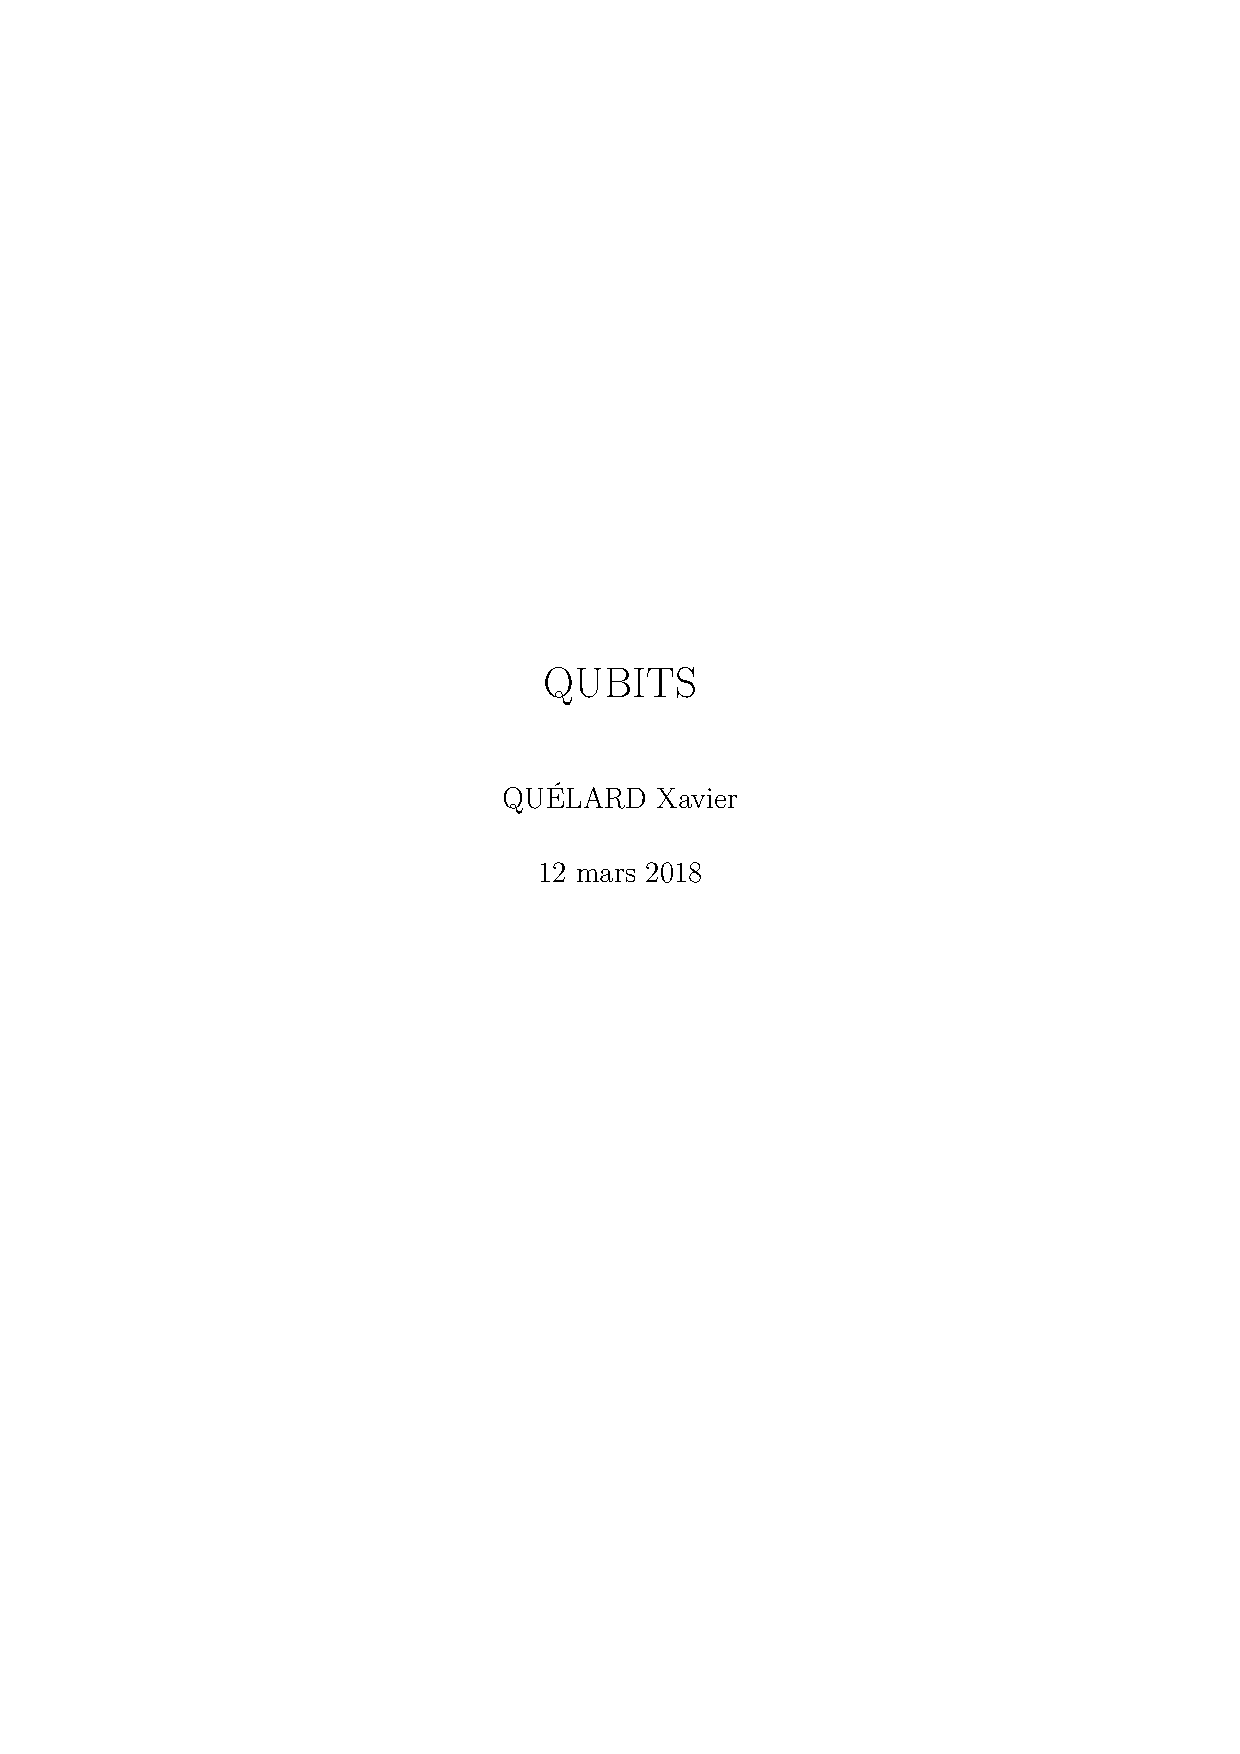
\includepdf[scale=0.8, pages=1-12, pagecommand={}]{french}

\end{document}
